\documentclass[12pt]{report}
%encoding
%--------------------------------------
\usepackage[T1]{fontenc}
\usepackage[utf8]{inputenc}
%--------------------------------------
 
%Portuguese-specific commands
%--------------------------------------
%\usepackage[portuguese, brazil, english]{babel}
%--------------------------------------
 
%Hyphenation rules
%--------------------------------------
\usepackage{hyphenat}
\hyphenation{mate-mática recu-perar}
%-----

\usepackage{graphics}
\usepackage{url}
\usepackage{lipsum}
\usepackage{graphicx}
\usepackage{geometry}
\usepackage{amssymb}
\usepackage{float}
\usepackage{verbatim} 
\usepackage{amsmath} 
\usepackage{amsfonts}
\usepackage{amssymb}
\usepackage{lmodern}
\usepackage[portuguese,ruled,lined]{algorithm2e}
\usepackage{algorithmic}
\usepackage{caption}
\usepackage{subcaption}
\usepackage{indentfirst}
\usepackage{mathrsfs,amsmath}
\usepackage{amstext}
\usepackage{hyperref}
\usepackage{setspace}
\usepackage[refpage]{nomencl}
\usepackage{nomencl}
\usepackage[alf,abnt-etal-cite=2,abnt-etal-list=0,abnt-etal-text=it,versalete,bibjustif]{abntex2cite}
\usepackage[alf]{abntex2cite}
\usepackage{epstopdf}
\usepackage{datetime}
\usepackage{booktabs}
%\usepackage[acronym]{glossaries}
%\usepackage{glossaries}
\usepackage{acro}
%\usepackage[acronym]{glossaries}
%\usepackage{longtable}
% probably a good idea for the nomenclature entries:
%\acsetup{first-style=short}
% class `abbrev': abbreviations:
%\DeclareAcronym{ny}{
%  short = NY ,
%  long  = New York ,
%  class = abbrev
%}
%\DeclareAcronym{la}{
%  short = LA ,
%  long  = Los Angeles ,
%  class = abbrev
%}
%\enableregime[utf]

\hypersetup{
    %bookmarks=true,         % show bookmarks bar?
    unicode=false,          % non-Latin characters in Acrobat’s bookmarks
    pdftoolbar=true,        % show Acrobat’s toolbar?
    pdfmenubar=true,        % show Acrobat’s menu?
    pdffitwindow=false,     % window fit to page when opened
    pdfstartview={FitH},    % fits the width of the page to the window
    pdftitle={My title},    % title
    pdfauthor={Author},     % author
    pdfsubject={Subject},   % subject of the document
    pdfcreator={Creator},   % creator of the document
    pdfproducer={Producer}, % producer of the document
    pdfkeywords={keyword1, key2, key3}, % list of keywords
    pdfnewwindow=true,      % links in new PDF window
    colorlinks=true,       % false: boxed links; true: colored links
    linkcolor=blue,          % color of internal links (change box color with linkbordercolor)
    citecolor=blue,        % color of links to bibliography
    filecolor=magenta,      % color of file links
    urlcolor=blue           % color of external links
}
\geometry{left=2.5cm, top=2cm, bottom=2.5cm, right=2cm}
\newcommand{\euler}{\textit{e}}
\newcommand{\complexSymbol}{\textit{j}}
\setstretch{1.5}

\hfuzz=30pt
%\vfuzz=20pt
\hbadness=2000
\vbadness=\maxdimen

\def\worktitle{Agrupamento de imagens de moda através de redes convolucionais artificiais}
\def\workauthor{Elvis Rafael Ferreira Dias}
\def\workadvisor{Agostinho de Medeiros Brito Júnior}

\usepackage{afterpage}

\newcommand\blankpage{%
    \null
    \thispagestyle{empty}%
    \addtocounter{page}{-1}%
    \newpage}

\acsetup{first-style=short}

% Exemplos de acrônimos, se necessários...
% class `abbrev': abbreviations:
\DeclareAcronym{DFT}{
  short = DFT ,
  long  = \textit{Discrete Fourier Transform} ,
  class = abbrev
}
\DeclareAcronym{IDFT}{
  short = IDFT ,
  long  = \textit{Inverse Fourier Transform} ,
  class = abbrev
}
\DeclareAcronym{FFT}{
  short = FFT ,
  long  = \textit{Fast Fourier Transform} ,
  class = abbrev
}

\DeclareAcronym{IFFT}{
  short = IFFT ,
  long  = \textit{Inverse Fast Fourier Transform} ,
  class = abbrev
}
\DeclareAcronym{2D DFT}{
  short = 2D DFT ,
  long  = \textit{Two-Dimensional Discrete Fourier Transform} ,
  class = abbrev
}

\providecommand{\keywords}[1]{\textbf{\textit{Keywords: }} #1}
\providecommand{\palavrasChaves}[1]{\textbf{\textit{Palavras-chaves: }} #1}

\newdateformat{monthyeardate}{%
  \monthname[\THEMONTH], \THEYEAR}
%%%%%%%%%%%%%%%%%%%%%%%%%%%%%%%%%%%%%%%%%%%%%%%%%%%%%%%%%%%%%
\begin{document}

%\selectlanguage{brazil}
\begin{titlepage}

	\centering
	{\normalsize \workauthor \par}
	%\includegraphics[width=0.15\textwidth]{example-image-1x1}\par\vspace{1cm}
	%{\scshape\LARGE Universidade Federal do Rio Grande do Norte \par}
	\vfill
	{\Large\bfseries \worktitle \par}
	\vfill

% Bottom of the page

	{\normalsize Brasil\par}
	{\normalsize \monthyeardate\today}
\end{titlepage}

\begin{titlepage}

	\centering
	{\normalsize \workauthor\par}
	%\includegraphics[width=0.15\textwidth]{example-image-1x1}\par\vspace{1cm}
	%{\scshape\LARGE Universidade Federal do Rio Grande do Norte \par}
	\vfill
	\centering
	{\Large\bfseries \par}
	\vfill

	\begin{flushright}	
	\begin{minipage}{15em}	
	\setstretch{1.0}
  	Trabalho de Conclusão de Curso Submetido à Coordenação do Curso de Engenharia de Computação e Automação do Centro de Tecnologia da Universidade Federal do Rio Grande do Norte, como parte dos requisitos necessários para a obtenção do grau de Engenheiro de Computação.
	\end{minipage}
	\end{flushright}	
	\vfill
	
	
	{\small Universidade Federal do Rio Grande do Norte - UFRN \par}
	{\small Coordenação do Curso de Engenharia de Computação e Automação - DCA \par}
	{\small Graduação em Engenharia de Computação \par}
	\vfill
	\normalsize
	\centering
	{\normalsize Orientador: Agostinho de Medeiros Brito Júnior \par}
	\vfill
% Bottom of the page
	{\normalsize Brasil\par}
	{\normalsize \monthyeardate\today}
\end{titlepage}

\pagenumbering{gobble}% Remove page numbers (and reset to 1)

%%%%%% AGRADECIMENTOS %%%%%%

\begin{center}
{\bf \Large Agradecimentos}
\end{center}



\newpage

%%%%%% RESUMO %%%%%%
\begin{abstract}

  \palavrasChaves{Movimento lento, Fluxo óptico, OpenCV, Shi-Tomasi,
    Triangulação de Delaunay}
    
\end{abstract}

\newpage

%%%%%% RESUMO EM INGLÊS %%%%%%
\selectlanguage{english}

\begin{abstract}
  abstract in english
  \\
  \keywords{translate-as}

\end{abstract}

\newpage

\selectlanguage{brazil}

%%%%%% LISTA DE FIGURAS %%%%%%

\listoffigures

\newpage

%%%%%% LISTA DE ABREVIAÇÕES %%%%%%

{\centering
\printacronyms[include-classes=abbrev,name=Abreviações]
}
\tableofcontents

%\makenomenclature
%\makeglossaries

%\newglossaryentry{DFT}{%
%name={DFT},%
%description={antigeen-presenterende cel}%
%}
\newpage

%%%%%% INÍCIO DO TEXTO %%%%%%

\pagenumbering{arabic}

\chapter{Introdução}
\label{cha:introducao}

Como estimado pela Forbes (2019), a indústria da moda chega a ser uma das maiores do mundo, chegando à movimentação de 3 trilhões em dólares em 2018. Embora muitas pessoas assumam que moda se resume a roupa, de certa forma até corretamente, moda consiste na verdade de um conceito muito mais complexo e significativo. Como definido pelo livro "Key Concepts for the fashion" (Reilly, 2014), moda é uma força intangível, manifestada em produtos tangíveis, representando novidade em relação a produtos passados; estes adotado por um grupo de pessoas, representando reflexos da cultura e sociedade. 

Para melhor entendimento é importante desassociar roupa, vestimenta e moda. Podemos pensar em roupa como uma peça têxtil confeccionada para ser usada no corpo. Já vestimenta inclui três elementos: (1) Qualquer elemento utilizado no corpo, por exemplo, roupas ou acessórios; (2) Qualquer modificação corporal, por exemplo, tatuagem e estilo de cabelo; (3) Qualquer atributo anexado ao corpo, seja uma bolsa ou muletas. 

Em geral toda vestimenta pode ser considerada semiótica, isto é, a forma como sinais podem ser vistos ou representados como uma ideia ou conceito, carregando consigo um significado determinado. Por exemplo, nos filmes de velho oeste americanos, o vaqueiro com chapéu branco é vestido pelo cara bom, enquanto que o cara mau veste o preto. A simbologia representada pela vestimenta neste caso faz com que as pessoas absorvam seu significado apenas ao ver as peças (Reilly, 2014).

Moda, por sua vez, remete a uma forma de vestimenta ou peça de roupa que se tornou, ou vai se tornar, popular; como foram os cabelos curtos para as mulheres na década de 20. Ainda, moda é um processo social, pois o que se torna popular nos grupos de pessoas tem influências culturais, assim como foi a moda dos anos 90 influenciada pela música da época. Por ser um processo moda vai além de itens vestíveis, podendo ser aplicado a outros tipos de indústria que não de roupa. O conceito de moda pode ser aplicado a qualquer objeto, comportamento ou modo de pensar. Existe moda no mundo automobilístico, moda nos animais que pessoas criam, até em qual tipo de rede social esta sendo utilizada (Reilly, 2014).

Na indústria da moda, as forças que moldam a aceitação popular influenciam também áreas além de roupas. Por exemplo, a escolha de joias varia com o mineral, material e design da peça. Maquiagem e unhas mudam de estilo de acordo com produtos, técnicas de aplicação e estética de forma geral. Seguindo de forma semelhante para calçados, cintos, lingeries, bolsas de mão, cortes de cabelo, etc (Reilly, 2014).

Moda é comumente encontrada relacionada a roupa devido a natureza da sua indústria e seus produtos. Vestimentas em geral, como roupas e acessórios, são mais práticas de serem criadas, produzidas e vendidas do que muitos outros produtos. Automóveis e mobílias, por exemplo, podem tomar anos de design e produção para chegar numa aceitação popular, sendo ainda por cima um processo caro para ser facilmente substituído. Ainda, outra explicação possível é o fato de roupa ser pessoal, estar próximo do corpo e estar vinculado a imagem corporal. Como Grogan (Grogan, 2008, 3) afirma, influenciando "a percepção, pensamentos e sentimentos de uma pessoa sobre seu corpo". A forma como uma pessoa percebe seu corpo afeta como ela se sentirá, consequentemente como se vestirá. Imagem corporal está diretamente associada com auto estima, levando o individuo insatisfeito com sua imagem a tomar atitudes para mudar este cenário. O que a indústria da moda procura portanto é manter esse sentimento nas pessoas. (Reilly, 2014)

Para cultura capitalista atual, produtos criados para moda ou como definição de moda, são pensados para terem uma vida útil curta. Modas são criadas para venderem em uma temporada, ter uma breve e próspera vida até ser descartada por algo novo. A obsolência programada que fundamenta a moda pode ser vista, portanto, de duas formas, aqui ilustrada em frases de grandes designers de moda: "Uma ótima moda é como um sexo casual; por ter uma vida curta, pode ser lembrada para sempre" -- Karl Lagerfeld; e "Uma arte difícil e frustrante, porque assim que o vestido nasce ele imediatamente se torna uma coisa do passado" -- Elsa Schiaparelli (Reilly, 2014).

O marketing necessário para fazer com que a moda não perca relevância no meio de tanta volatilidade intencional, é também muito forte. Em anos pré-guerras produtos já eram comercializados com a ajuda de imagens e catálogos. A imagem do produto era o mais importante, sendo vinculado ao status de posse (Cultural History of Fashion). Como afirma fashionista, designers começaram a contratar mulheres para vestir seus designs caminhando em eventos como corridas de carro para possibilitá-las serem percebidas, fotografadas e reportadas na mídia. A partir disso, não demorou muito para que estas exibições se tornassem concentradas em um ambiente fechado para um público específico, ganhassem cara de evento social importante e começassem a serem agendadas em datas fixas no ano (fashionista).

Com o aumento da quantidade de eventos para apresentação de designs e aumento da credibilidade, designers no início do século passado já contavam com audiência indo do mundo todo para a França em períodos agendados. Este estilo das apresentações foi adotado como padrão e mantido por quase todo o século, sendo caracterizado por modelos caminhando por um percurso envolto de audiência, formada por clientes e jornalistas responsáveis por fazer a moda atingir um grande alcance através de sua divulgação (fashionista). O jornalismo de moda cobre todos os tipos de mídia sobre a indústria da moda, desde pessoas que constroem este mundo até a moda usável em si (Fashion Jornalism), fazendo com o público possa se preparar para comprar na temporada seguinte assim como empresas e designers tenham tempo para produção em larga escala. 

Entretanto, como a vogue do Reino Unido afirmou, esta dinâmica secular precisa ser repensada. A ideia do mundo ver coleções de novas vestimentas e tendências como algo para o futuro não tem mais feito sentido no mundo moderno das redes sociais. Atualmente a dependência dos jornalistas para que os novos designs ganhem escala mundial não existe mais, assim como o poder da imagem se tornou mais momentâneo do que nunca antes, podendo perder seu valor antes que os clientes possam realmente comprar. 
A ideia tem sido capitalizar em cima do \textit{buzz} gerado pelas redes sociais com os eventos de moda, aumentando a relevância dos designs enquanto o interesse dos clientes não é comprometido pelo tempo (VOGUE UK, 2016).   

%Analyzing fashion attributes is essential in fashion design process. Current fashion forecasting firms, such as WGSN utilizes information from all around the world (from fashion shows, visual merchandising, blogs, etc) [1–3]. They gather information by experience, by observation, by media scan, by interviews, and by exposed to new things. Such information analyzing process is called abstracting, which recognize similarities or differences across all the garments and collections. In fact, such abstraction ability is useful in many fashion careers with different purposes [4]. Fashion forecasters abstract across design collections and acrosstime to identify fashion change and directions; designers, product developers and buyers abstract across group of garments and collectionsto develop a cohesive and visually appeal lines; sales and marketing executives abstract across product line each season to recognize selling points; fashion journalist and bloggers abstract across runway photos to recognize symbolic core concepts that can be translated into editorial features[5]. (A Deep-Learning-Based Fashion Attributes Detection Model)

Apesar da natureza bem estabelecida e sólida da industria da moda, inteligência artificial (IA) tem traçado seu caminho por esta transformando-a de diferentes formas, desde a fabricação dos seus produtos até a forma com que seus produtos são usados em propagandas e vendidos. Segundo a Forbes, IA está transformando a indústria da moda em todos os elementos que compõem sua cadeia, tais como design, fabricação, logística, marketing e vendas (FORBES ,2018).

Nas vendas, tecnologias de IA tem maximizado a experiência de compra dos consumidores e tornado os sistemas mais eficientes através de análise preditiva para companhias conseguirem guiar suas vendas ou preverem tendências. Para citar alguns exemplos de experiências dos usuários, consumidores agora podem tirar fotos de roupas que gostam ou estilos que querem imitar e sistemas inteligentes se responsabilizam para encontrar itens relacionados a venda. Ainda, saber quais itens uma imagem, roupas e acessórios, são compráveis e onde achá-los ou obter um serviço de estilista no próprio smartphone baseado em inteligência artificial (FORBES, 2018).

\section{Objetivos}

Estamos vivendo em uma época que tecnologias de inteligência artificial podem agregar valor em qualquer parte da indústria da moda, sendo afirmado que "O futuro da moda é inteligente" (FORBES, 2018). Sendo assim, foi pensado em uma ferramenta para ajudar consumidores e jornalistas a analisarem coleções e tendências de forma prática e rápida, a partir da organização inteligente de imagens de moda em formato de painéis, a partir de suas características, de forma automática. 

O processo de análise de coleções de moda pode tomar muito tempo, entusiastas, por exemplo, têm dezenas de desfiles por temporada de moda gerando centenas de imagens várias vezes ao ano. Jornalistas, responsáveis por diluir toda essa informação e filtrar para o público com senso cultural, precisam de velocidade e alto conhecimento para gerar informação rápida sobre os shows. 

A ferramenta, fundamentada em inteligência artificial, propõe analisar imagens de moda e distribui-las em um espaço 3-d e 2-d, de forma que a distância entre as imagens represente a similaridade, se próximas, ou dissimilaridade, se distantes. O algoritmo leva em conta diversas formas de texturas, formas, padrões a fim de achar como as imagens podem ser melhor vista e analisadas juntas. 

Neste ponto a análise das coleções passa a ser em conjunto, como melhor devem ser, de forma a formar uma linha coerente, ao invés de imagens soltas desassociadas. Este tipo de visão espacial pode ajudar na geração de "insight" se várias imagens se mostram muito próximas entre si e distantes de outros grupos e ainda, por fim, possibilita a facilidade na comparação de coleções de diferentes designers, de diferentes anos ou diferentes temporadas, podendo criar um glossário onde características marcantes das coleções são armazenadas e usadas posteriormente para comparação e estudo em geral.

\chapter{Fundamentação teórica}
\label{cha:fund-teor}

Dentre as ferramentas utilizadas para desenvolvimento do projeto, está o uso de imagens digitais, visão computacional, redes neurais convolucionais, aprendizado de máquina profundo e algoritmos de agrupamento por redução dimensional. Nesta seção estes tópicos são explicados com viés de aplicação neste projeto, afim de facilitar a imersão do leitor no entendimento do desenvolvimento.

\section{Visão Computacional}

Seja em um computador ou em um animal, visão é composta de dois componentes: Sensor e interpretador. O sensor sendo uma câmera ou o olho que captura luz e transmite como informação para o interpretador que trará significado a informação obtida, sendo este o cérebro ou sistemas especialistas. Esta área de estudo é considerada muito difícil de ser resolvida devido a dificuldade de associar valores discretos de uma imagem com significado. Traçar o significado, por exemplo, para uma imagem digital colorida com tamanho 200x200 pixels de largura e altura respectivamente, composta por uma combinação de 120.000 valores possíveis, não é simples. (Stanford, 2017)

Portanto, visão computacional pode ser definido como um campo de estudo científico dedicado a extração de informações de imagens digitais. A extração pode ser feita através de algoritmos e utilizados em diversas aplicações, uma vez que o tipo de informação ganha de uma imagem podem ser de dois tipos: Medições ou semântica. Neste trabalho a visão computacional será abordada sob a perspectiva semântica, isto é, rótulo de objetos ou de cenas em uma imagem, reconhecimento de pessoas, gestos ou faces, etc. (Stanford, 2017)

Imagens digitais tem como base a convenção de um dos inventores da escaneadora: Russel Kirsch (NIST). A convenção batizada com seu nome, define imagem digital como uma função bidimensional de intensidade de luz $f(x, y)$ onde $x$ e $y$ denotam coordenadas espaciais e o valor dado pela função em qualquer ponto é chamado de intensidade da imagem neste ponto (pixel, se pensado em uma tela \textit{display}). Quando os valores de $x$, $y$ e da intensidade são todos finitos portanto, $f$ pode ser chamado de imagem digital (GONZALEZ; WOODS, 2012). 

Em casos de imagens preto e branco o valor desta intensidade se faz de um valor inteiro, enquanto que para imagens coloridas cada intensidade é representada por um vetor tridimensional, como ilustra a figura \ref{fig:repre-imgs}. Existem alguns modelos para representar imagens coloridas digitalmente, por exemplo, no modelo RGB (do inglês \textit{Red Green Blue}) a unidade de intensidade é composta pela mistura da intensidade destas três cores primárias; ou seja, essa mistura é capaz de gerar todas as cores mostradas por uma tela (GONZALEZ; WOODS, 2012). 

%\begin{figure}
%  \begin{subfigure}{\linewidth}
%  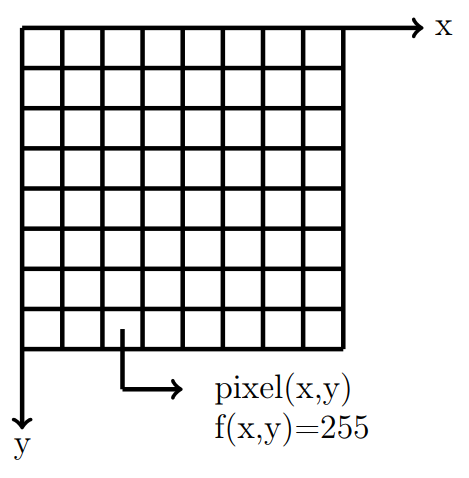
\includegraphics[width=.3\linewidth]{images/dig-img1.png}\hfill
%  \centering
%  \caption{Imagem preto e branco}
%  \label{fig:dig-img1}
%  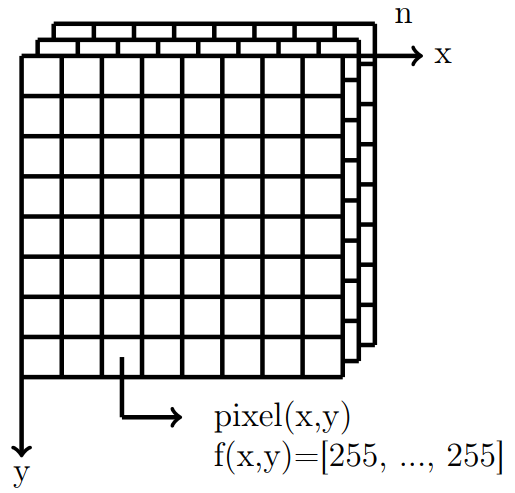
\includegraphics[width=.3\linewidth]{images/dig-img2.png}\hfill
%  \centering
%  \caption{Imagem colorida}
%  \label{fig:dig-img2}
%  \end{subfigure}\par\medskip
%  \caption{Representações de imagens digitais}
%\end{figure}

\begin{figure}
  \centering
  \begin{minipage}[b]{0.4\textwidth}
    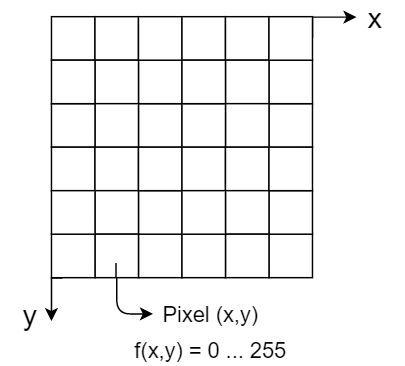
\includegraphics[width=\textwidth]{images/imagembew.png}
    \caption{Imagem preto e branco}
  \end{minipage}
  \hfill
  \begin{minipage}[b]{0.4\textwidth}
    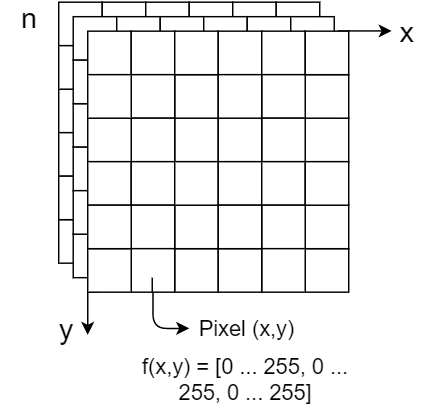
\includegraphics[width=\textwidth]{images/imagemcolorida.png}
    \caption{Imagem colorida}
  \end{minipage}
  \caption{Representação de imagens digitais}
  \source{}
  \label{fig:repre-imgs}
\end{figure}

\subsection{Filtragem Espacial de Imagens Digitais}

O processo de filtragem de uma imagem digital refere-se ao processo de transformação dos valores de intensidade dos pixels a partir dos seus vizinhos, dando assim origem a uma nova imagem. O filtro é feito a partir da operação da convolução digital de \textit{kernels} fixos sob todos os pixels da imagem e tem como propósito a geral extração de informações específicas da imagem, por exemplo, detecção de bordas, projetando-as na nova imagem (Stanford, 2017).

Um exemplo intuitivo para entendimento é a média móvel, filtro que torna o valor de um pixel central a média dos seus pixels vizinhos. Definido matematicamente como $g[m,n] = \frac{1}{9} \sum_{i= -1}^{1} \sum_{j= -1}^{1} f[m - i,n - j]$, ilustrado na figura \ref{fig:blur}, a média móvel suaviza as bordas marcantes de uma imagem, criando um efeito de borrão sob a mesma (Stanford, 2017).  

\begin{figure}
    \centering
    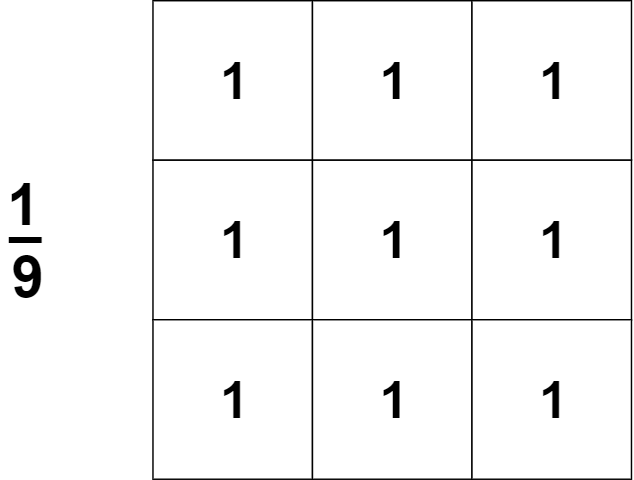
\includegraphics[width=0.35\textwidth]{images/blur.png}
    \caption{Kernel da média móvel}
    \source{} 
    \label{fig:blur}
\end{figure}

\subsubsection{Operação da convolução}

Como mencionado, esta operação usa informação de pixels vizinhos para junto com um \textit{kernel} para transformar a intensidade de um pixel alvo. GoodFellow et al. (2016) ilustra este conceito a partir de um laser mantendo a localização de um nave espacial. O laser fornece uma única saída $x(t)$, a posição da nave no tempo $t$, podendo ser lido a qualquer instante de tempo. Agora imagina-se que o laser está em uma região ruidosa, para obtenção de uma estimativa menos ruidosa da posição é interessante fazer uma média de várias medições recentes. Para priorizar medidas recentes, esta média precisa associar estas a um peso maior, fazendo assim uma média ponderada $w(a)$, com a idade da medição. Se esta operação é aplicada a cada momento, é obtido portanto uma função \textit{s}, fornecendo uma posição suavizada da espaçonave:

\begin{equation}
    s(t) = \int x(a)w(t - a)da
\end{equation}

Esta operação linear é denominada portanto convolução, por padrão escrita pelo símbolo * como $s(t) = (x * w) (t)$ (GOODFELLOW et al, 2016).

No exemplo ilustrativo acima \textit{w} precisa ser uma função densidade de probabilidade válida e 0 para todos os argumentos negativos, não valendo para o futuro. Ainda, o tempo válido para qualquer instante não é realístico. Esta operação, se feita em um computador, terá seu tempo discretizado, isto é, o sensor enviaria dados apenas em um intervalo regular de tempo. Pode-se assumir ainda que o tempo de medição é valido para valores inteiros, assim com \textit{x} e \textit{w} definidos apenas para \textit{t} inteiro, pode-se escrever a convolução discreta como (GOODFELLOW et al, 2016):

\begin{equation}
    s(t) = (x*w)(t) = \sum_{a = -\infty}^\infty x(a)w(t - a)
\end{equation}

A convolução discreta pode ser vista portanto como multiplicação de matrizes, sendo uma dessas matrizes variante porém sempre com o mesmo tamanho. Como ilustra a figura \ref{fig:convo}, utilizando a terminologia de redes neurais convolucionais (Explicadas em outra seção), o primeiro argumento da convolução (nosso \textit{x} do exemplo) refere-se a imagem de entrada, ou \textit{input}, o segundo argumento (a função \textit{w}) como o \textit{kernel} e a saída como mapa de características, do inglês \textit{feature map}. Dessa forma, o \textit{kernel} desloca-se pela imagem fazendo operações de multiplicação e soma que resultarão no resultado da convolução. 

\begin{figure}
    \centering
    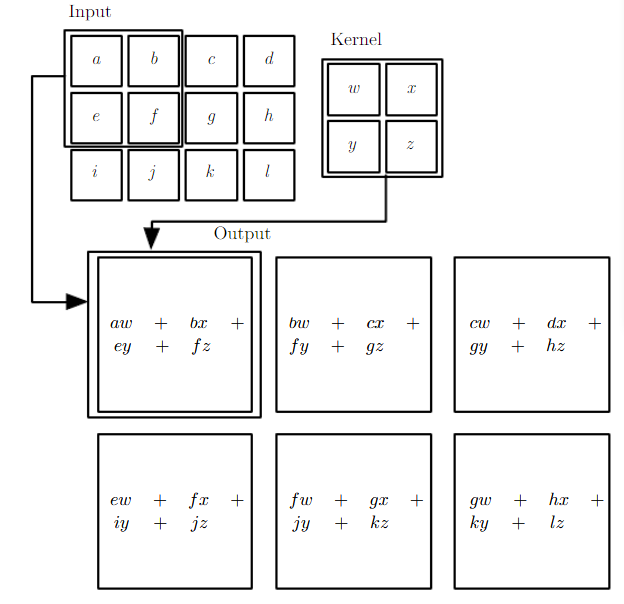
\includegraphics[width=0.65\textwidth]{images/convo.png}
    \caption{Um exemplo de convolução 2-d. As setas apontam para o resultado de uma única operação de convolução, sobre a parte superior esquerda da imagem, ao qual utiliza 4 pixels para gerar apenas um novo}
    \source{Source: dps} 
    \label{fig:convo}
\end{figure}

No exemplo a operação varre todo o \textit{input} de tamanho 4x3 pixels com um \textit{kernel} de tamanho 2x2, resultando em uma imagem 3x2. Entretanto, a detecção de características significantes é melhor feita quando o \textit{kernel} não varre todos os pixels da imagem ou com \textit{kernels} de tamanho maior (técnica chamada interações esparsas, do inglês \textit{Sparse Interactions}). Ainda, a redução de dimensionalidade apresentada na saída se comparado com a entrada se faz benéfico para sistemas de visão computacional em geral e será melhor discutido na sessão de redes neurais convolucionais (GOODFELLOW et al, 2016).

\subsection{Segmentação de Imagens Digitais}

Segmentação de imagens é um processo de categorizar cada pixel em uma imagem, tal que pixels com o mesmo rótulo possuam a mesma propriedade semântica (GHOSH et al, 2019). Humanos conseguem fazer segmentação de pixels de forma intuitiva, por exemplo, em uma imagem de uma rua saber qual região de pixels correspondem a rua, pessoas e carros, porém o para um computador conseguir atribuir significado a pixels juntos leva-se um pouco mais de esforço (Stanford, 2017).  

A segmentação de imagens digitais pode ser entendido como uma evolução natural de classificação de imagens, que consiste em um sistema fazer uma previsão correspondente a uma entrada, neste caso uma imagem inteira. Localização e detecção são os passos seguintes para o aperfeiçoamento desta visão computacional, percebendo informações adicionais sobre localização espacial de elementos da imagem. Naturalmente, após conseguir detectar elementos no espaço, surge a segmentação semântica, categorização de todos os pixels em classes. Por fim, o maior nível de aperfeiçoamento consiste da segmentação de instância, categorização dos itens de uma mesma classe, como representados na figura \ref{fig:seg} (Garcia-Garcia, 2017).

\begin{figure}
  \centering
  \begin{minipage}[b]{0.4\textwidth}
    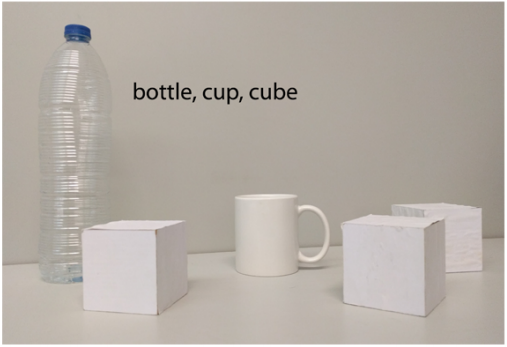
\includegraphics[width=\textwidth]{images/seg1.png}
    \caption{Classificação da imagem}
  \end{minipage}
  \hfill
  \begin{minipage}[b]{0.4\textwidth}
    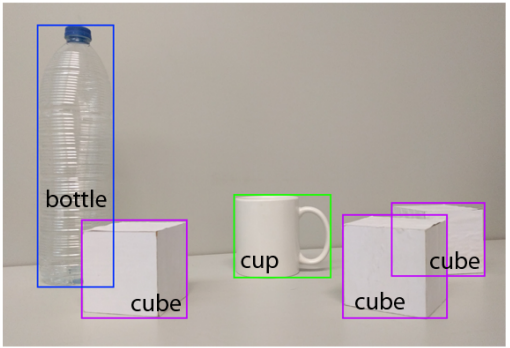
\includegraphics[width=\textwidth]{images/seg2.png}
    \caption{Localização de objetos}
  \end{minipage}
    \hfill
  \begin{minipage}[b]{0.4\textwidth}
    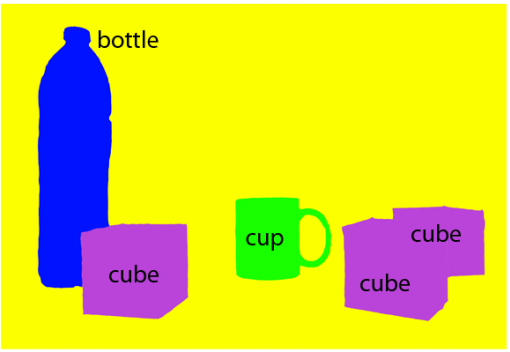
\includegraphics[width=\textwidth]{images/seg3.png}
    \caption{Segmentação semântica}
  \end{minipage}
    \hfill
  \begin{minipage}[b]{0.4\textwidth}
    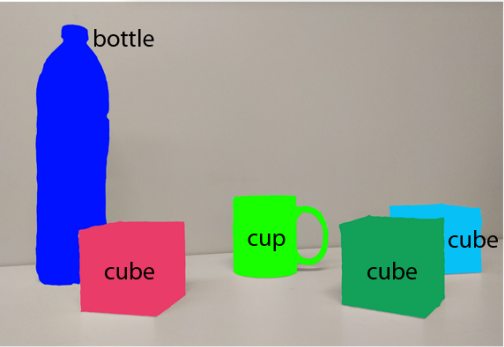
\includegraphics[width=\textwidth]{images/seg4.png}
    \caption{Segmentação de instância}
  \end{minipage}
  \caption{Evolução do entendimento de cenário desde uma inferência grosseira até uma mais refinada: classificação, detecção ou localização, segmentação semântica e segmentação de instância.}
  \source{Source: dps}
  \label{fig:seg}
\end{figure}

Técnicas para segmentação de cenas digitais não são recentes, porém sua popularidade foi revolucionada pelo aprendizado de máquina profundo. Ferramentas como redes neurais convolucionais permitiram que esta área da visão computacional fosse aplicada de diversas formas, como em carros autônomos, iteração homem máquina, na busca inteligente de imagens e realidade aumentada para nomear algumas (Garcia-Garcia, 2017). Mais a frente será discutido como o aprendizado de máquina trouxe tanto poder para este campo de estudo e como este trabalho faz uso de segmentação de instâncias.

\subsection{Redução de Dimensionalidade}

Na visão computacional é de grande importância a utilização de ferramentas capazes de reduzir a quantidade de características usadas para descrever os dados. A redução de dimensionalidade consiste de uma área de estudo capaz de transformar representações de dados com fim de buscar melhorar a performance de algoritmos de visão computacional, assim como de modelos baseados em aprendizado de máquina em geral (Stanford, 2017). Dentre os métodos existentes, destacaremos aqui a análise de componentes principais (do inglês \textit{Principal Component Analysis} - PCA) e \textit{t-Distributed Stochastic Neighbor Embedding} (t-SNE).

\subsubsection{Estatística Necessária}

O campo da estatística procura analisar relação entre os dados de um conjunto. Medições de dispersão da distribuição dos dados como desvio padrão ou variância dos dados podem ser feitas em dados unidimensionais, portanto, muitos conjuntos de dados possuem múltiplas dimensões. Nesses casos, portanto, a covariância se mostra útil para analisar como uma dimensão varia de acordo com a média, em relação a outra dimensão. Esta medida é sempre feita para duas dimensões e pode ser vista abaixo (SMITH, 2002):

\begin{equation}
    cov(x, y) = \sigma(x,y) = \frac{\sum_{i=1}^{n}(x_i - \overline{x})(y_i - \overline{y}}{(n - 1)}
\end{equation}

Para ilustrar imagina-se duas dimensões: horas estudadas (H) e nota recebida (N). O valor absoluto do cálculo \textit{cov(H,N)} não tem muito significado quanto seu sinal: se o valor for positivo, indica que ambas as dimensões aumentam juntas; caso contrário, as horas de estudo resultaria em notas piores. Ainda, se a covariância for 0 indica que as duas dimensões são independentes entre si (SMITH, 2002).

Como a covariância é uma medida bidimensional, se os dados existirem em mais dimensões a covariância será calculada diversas vezes. Por exemplo, para um conjunto de dados nas dimensões x e y, podemos calcular \textit{cov(x,x)}, \textit{cov(x,y)}, \textit{cov(y,x)}, \textit{cov(y,y)}, levando a matriz $ \sum = \begin{bmatrix}
    \sigma(x,x) & \sigma(x,y)\\
    \sigma(y,x) & \sigma(y,y)
    \end{bmatrix}
$. Dessa forma, uma matriz de covariância pode ser escrita contendo todos os cálculos de covariância para um determinado conjunto de dados. Para uma quantidade n de dimensões, podem ser calculadas $\frac{n!}{(n-2)!*2}$ covariâncias diferentes (SMITH, 2002).

Considere o exemplo que ilustra a distribuição dos dados no espaço bidimensional ilustrado pela figura \ref{fig:corr_2d}. Neste, os pontos x e y são correlacionados, com matriz de covariância  $ \sum = \begin{bmatrix}
    16.87 & 14.95\\
    14.94 & 17.27
    \end{bmatrix}
    $
. Neste caso, a orientação dos dados na diagonal é capturado pela covariância, enquanto que o espalhamento nos sentidos dos eixos são capturados pela variância. Portanto, qualquer vetor que direciona a distribuição dos dados (variância) é chamado de autovetor, enquanto que seu autovalor corresponde a variação ao longo deste vetor (DUMMY, 2014) . 

\begin{figure}
    \centering
    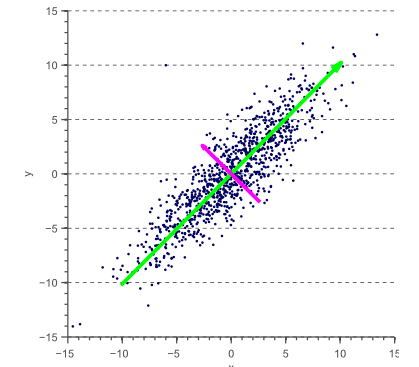
\includegraphics[width=0.5\textwidth]{images/correlated_2d.png}
    \caption{Dados correlacionados em duas dimensões com autovetores ilustrados em cores}
    \label{fig:corr_2d}
    \source{Fonte: dps}
\end{figure}

A partir da relação direta da matriz de covariância com uma transformação linear de dados aleatórios não relacionados, esta matriz pode ser reescrita como uma sequência de rotações definidas por seus autovetores. Dessa forma, os dados da figura acima podem ser reescritos de forma descorrelacionada rotacionando cada ponto, de forma a fazer com que os novos eixos de referência sejam seus autovetores (DUMMY, 2014). 

\subsubsection{Análise de Componente Principal (PCA)}

Se imaginar um conjunto de características descrevendo dados alvos de estudo após um processamento de visão computacional e sabendo que usar todas as característica não se mostra uma solução ótima devido o comprometimento de performance computacional e capacidade de aprendizado de modelos inteligentes, a dúvida que surge é: qual destas características devem ser priorizadas e quais destas podem ser removidas sem perder informações importantes? (DUMMY, 2014) 

Se as características fossem estatisticamente independentes, bastaria eliminar as menos relevantes, porém na prática muitas características dos dados são dependentes entre si, fazendo com uma única característica possa representar múltiplos tipos de informação. PCA portanto surge como uma possível solução para este problema, realizando uma transformação do espaço das características para obter informações descorrelacionados (DUMMY, 2014).

De forma intuitiva PCA pode ser pensado da seguinte forma: Digamos que é desejado diferenciar ingredientes de comida baseando-se em seus componentes nutricionais. Qual variável será suficientemente boa para diferenciar? Se a variável varia muito de um ingrediente para outro, será possível isolar bem os ingredientes, enquanto que mais difícil caso contrário. Quando os dados não apresentam uma variável que os separe bem, pode ser criado uma variável artificial a partir de combinações lineares de variáveis originais. Essencialmente PCA acha a melhor combinação linear das variáveis originais para que a variância com relação a nova variável seja máxima (Paper space, 2017).

\begin{figure}
  \centering
  \begin{minipage}[b]{0.4\textwidth}
    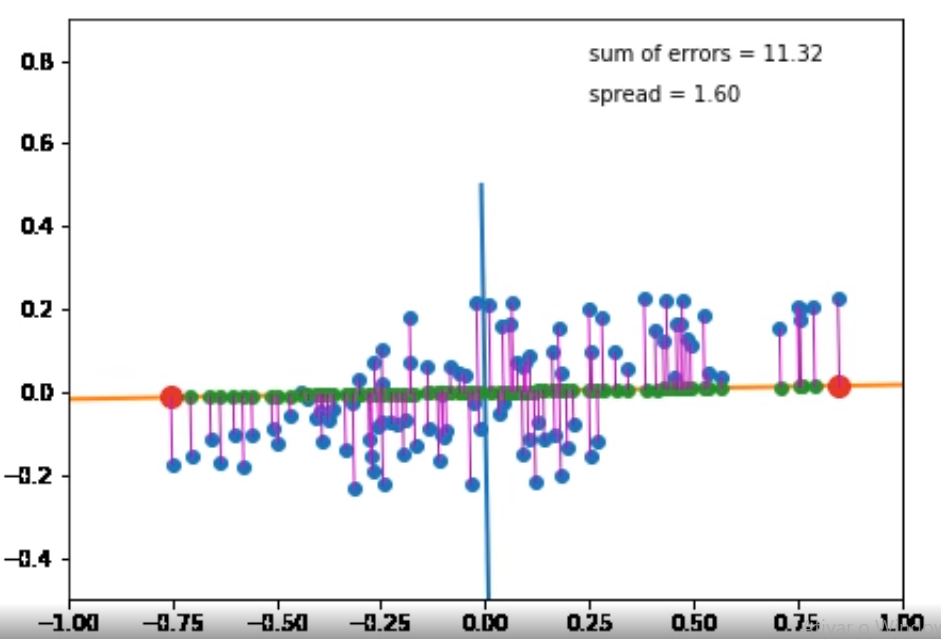
\includegraphics[width=\textwidth]{images/1.png}
  \end{minipage}
  \hfill
  \begin{minipage}[b]{0.4\textwidth}
    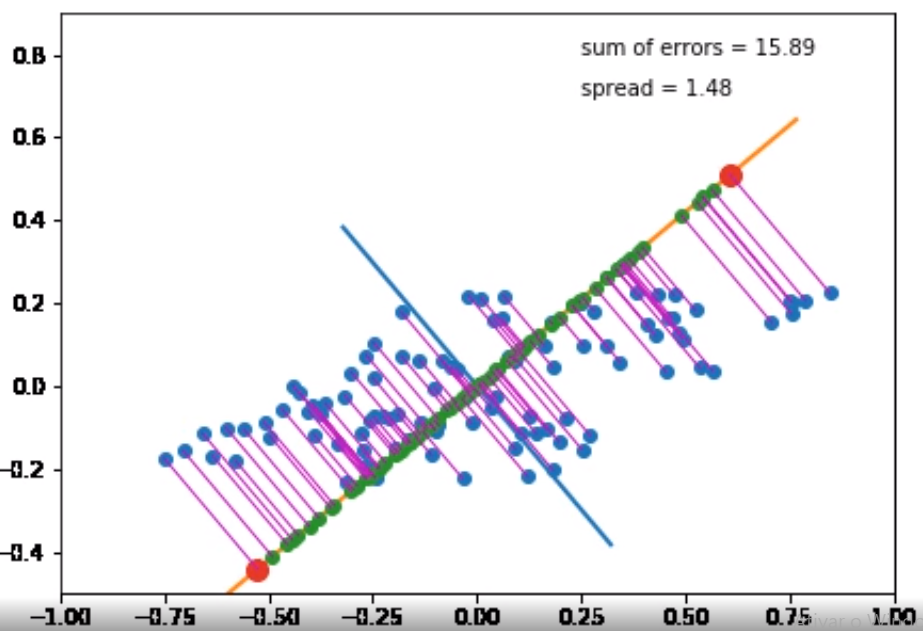
\includegraphics[width=\textwidth]{images/2.png}
  \end{minipage}
    \hfill
  \begin{minipage}[b]{0.4\textwidth}
    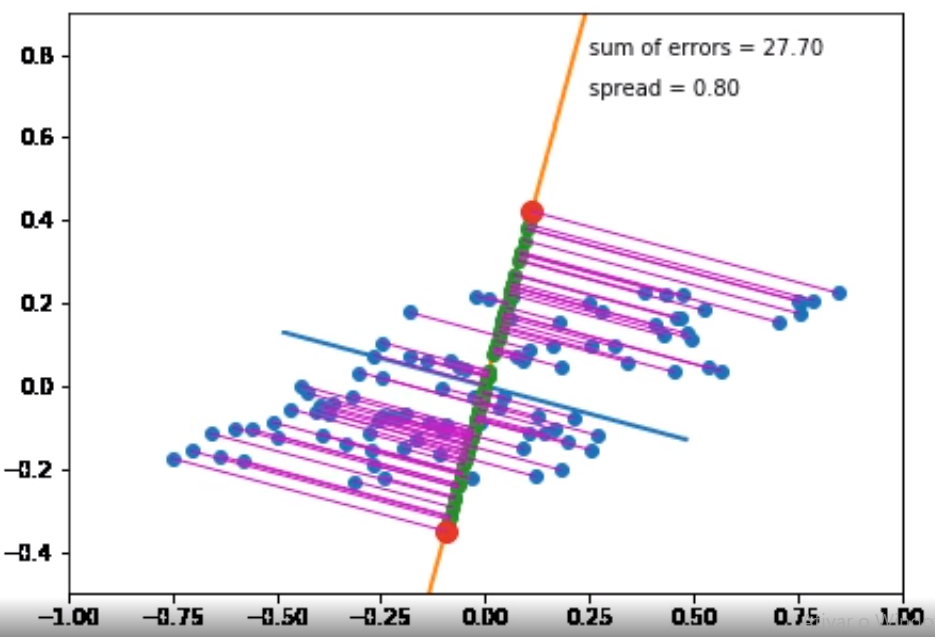
\includegraphics[width=\textwidth]{images/3.png}
  \end{minipage}
    \hfill
  \begin{minipage}[b]{0.4\textwidth}
    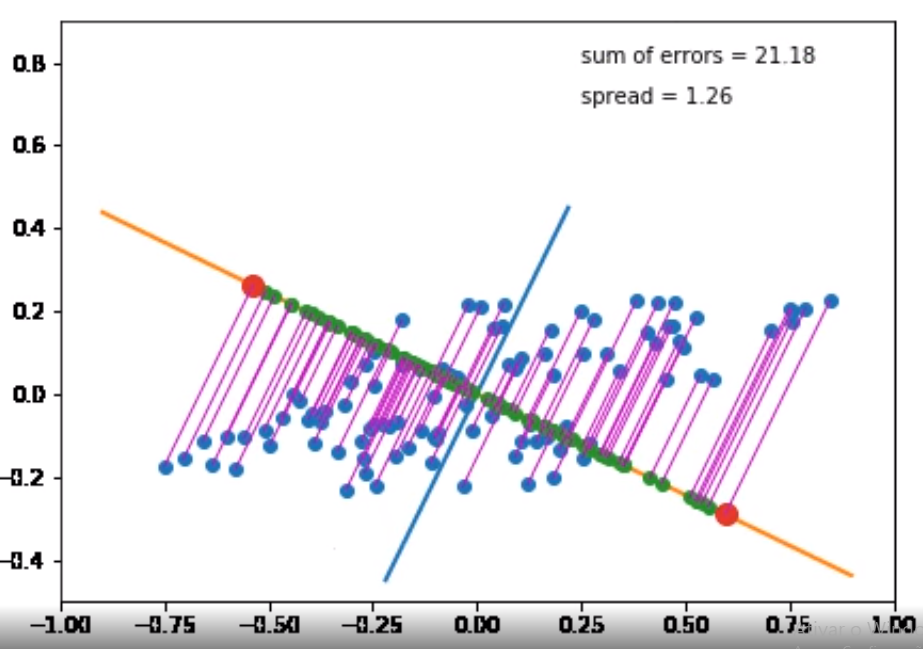
\includegraphics[width=\textwidth]{images/5.png}
  \end{minipage}
  \caption{Ilustração de um vetor variando no espaço em busca da maior variância do dados projetados sobre si.}
  \source{Fonte: dps}
  \label{fig:animacao_pca}
\end{figure}

Na figura \ref{fig:animacao_pca} cada ponto azul representa um ponto de informação representado pelas coordenadas (x,y). A linha laranja L é desenhada no centro dos dados (por exemplo, na média de x e y) e todos os pontos são projetados sobre esta linha, gerando os pontos verdes. A variância dos dados ao longo da linha é dada pela distância entre os pontos vermelhos, que enquanto L rotaciona esta distância muda de acordo com o ângulo criado entre L e o eixo X. As linhas roxas que ligam os pontos representam o erro do ponto real para a sua projeção e como PCA cria novas variáveis a partir de existentes, espera-se que este erro seja pequeno para que as novas variáveis sejam mais próximas possíveis das originais (Paper space, 2017).

A soma quadrada dos comprimentos de todas as linhas roxas fornece portanto o erro total de aproximação. O ângulo que minimiza a soma quadrada, também maximiza a distância dos pontos vermelhos, garantindo que os pontos que são distantes no plano original, continuem distantes no plano transformado; o vetor que maximiza a variância é chamado eixo principal. Após obter o eixo principal portanto, o método refaz o processo sobre variância restante com relação ao novo eixo para achar o próximo eixo principal. 

Uma vez que todos os eixos principais são encontrados, os dados são projetados nesses eixos, chamados agora de componentes principais. A redução de dimensões em si acontece após o cálculo dos autovalores e autovetores, projetando os dados sempre nos maiores autovetores. A relevância de um autovetor para ser um possível escolhido como eixo principal é medida a partir do autovalor associado, quanto maior o autovalor do autovetor mais informação aquele autovetor possui sobre o dado (Paper space, 2017).

Neste trabalho PCA será utilizado para reduzir dimensão de características sobre imagens digitais de moda. Na próxima seção, será falado como redes neurais convolucionais leem características de imagens digitais e geram essa representação em alta dimensão. Para torná-las úteis para utilização em um algoritmo que classifique estas imagens se faz necessário reduzir a dimensão e tentar descartar eventuais dados irrelevantes. 

\subsubsection{t-Distributed Stochastic Neighbor Embedding (t-SNE)}

Técnicas de visualização são essenciais para aplicações com dados, entretanto a maioria das técnicas de visualização podem somente serem aplicadas para inspeção de um número limitado de variáveis de interesse simultaneamente. Dessa forma, estas técnicas não são aplicáveis a projetos de grandes quantidades de dados que são multidimensionais (Google Tech Talk, 2013).

Uma forma efetiva de visualizar dados multi-dimensionais é representar cada objeto de informação como um ponto 2-d, de forma tal que informações semelhantes sejam representadas por pontos próximos no espaço e objetos não similares representados por pontos distantes. Este mapeamento de informação em pontos no espaço leva a construção de um mapa dos dados, possibilitando revelar melhor sua estrutura e até possíveis presença de aglomerados de dados similares (Google Tech Talk, 2013). 

\begin{figure}
    \centering
    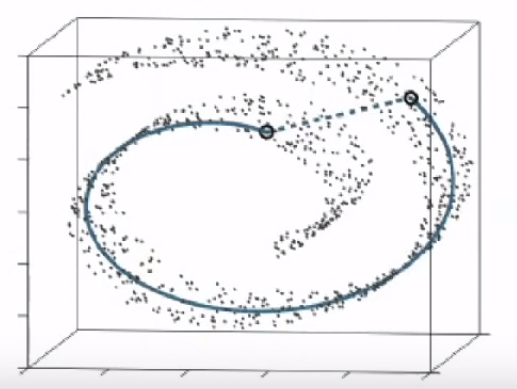
\includegraphics[width=0.4\textwidth]{images/pca.png}
    \caption{Comparação de amostras no espaço se comparando distância ou contexto estrutural.}
    \label{fig:pcaxtsne}
    \source{Fonte:}
\end{figure}

Para realizar tal feito, é necessário minimizar uma função que meça a discrepância entre as similaridades nos dados originais e nos dados mapeados. Na figura \ref{fig:pcaxtsne} se considerarmos a distância entre amostras para media sua correlação, assim como PCA faz, forneceríamos um entendimento errôneo para a visualização, pois o mais importante para medir correlação nesta imagem é sua forma. Por conta deste problema da distância PCA não serve para visualização, na imagem os pontos seriam semelhantes devido a posição, porém se olharmos para a estrutura eles são muito diferentes (MAATEN, 2013).

A técnica mais eficiente para embutir dados multi-dimensionais em uma visualização bidimensional ou tridimensional é abreviada por t-SNE. Esta mede em altas dimensões mede a densidade de um ponto com relação apenas a seus vizinhos e a partir de uma função de minimização garante que esta densidade será igual em menos dimensões (figura \ref{fig:xdto2d}). O cálculo em baixa dimensão é feito colocando os pontos em lugares aleatórios até que através de um cálculo repetitivo seja encontrado uma distribuição de pontos com densidades semelhantes dimensionalmente (MAATEN, 2013). 

\begin{figure}
    \centering
    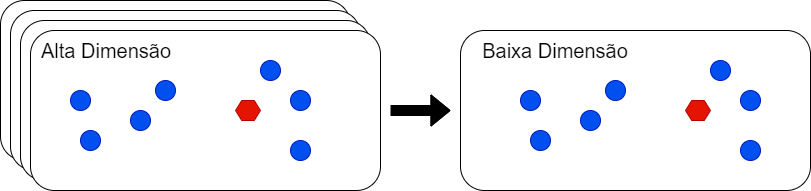
\includegraphics[width=0.8\textwidth]{images/xdto2d.png}
    \caption{Mapeamento de dados de alta dimensão para baixa dimensão preservando a densidade de distribuição das amostras}
    \label{fig:xdto2d}
    \source{Fonte: Baseada na ilustração do MAATEN (2013)}
\end{figure}

O autor desta técnica ilustra seu potencial para imagens a partir de amostras de números. Após processar as imagens através de um modelo inteligente obtém-se uma grande quantidade de características descritivas para cada amostra. A técnica é utilizada portanto para visualização em duas dimensões das características em altas dimensões. A figura \ref{fig:tsne} ilustra o resultado obtido onde todas as amostras de imagens referentes a um número são visualizadas próximas de si, com distância para as outras amostras de acordo com a similaridade dos números (MAATEN, 2013).  

\begin{figure}
    \centering
    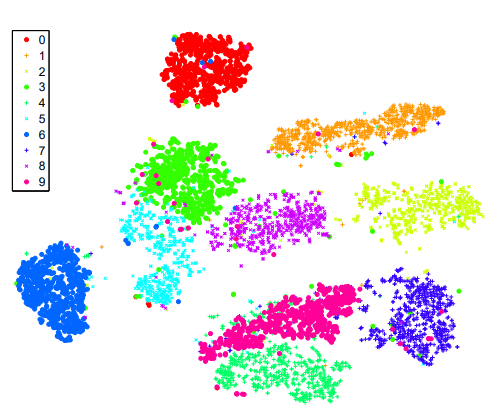
\includegraphics[width=0.6\textwidth]{images/ts.png}
    \caption{Exemplo de visualização utilizando t-SNE aplicado a imagens de número. Este não só mostra as diversas amostras de imagens aglomeradas por classe como também preserva em duas dimensões a distância entre as classes baseando-se em suas características descritivas.}
    \label{fig:tsne}
    \source{Fonte: dps}
\end{figure}


\section{Aprendizado de máquina}

Algoritmo de aprendizado de máquina são algoritmos capazes de aprender a partir de dados. Mitchell (1997) define aprendizado como um programa de computador que ao ter aprendido a fazer tarefas T com performance P baseado em uma experiência E, consiga melhorar sua performance P em T a partir desta experiência E. Aprendizado é o sentido atribuído ao alcance da habilidade de performar a tarefa (GOODFELLOW et al, 2016).

Em aprendizado de máquina o objetivo é fazer com que os algoritmos, também  chamados de modelos, generalizem seu aprendizado, sob um conjuntos de dados, em dados nunca antes visto. Dessa forma, os dados a serem fornecidos ao modelo devem ser separados em três conjuntos: Treinamento, validação e teste (Chollet, 2017). Os dados de treinamento são separados em dois, geralmente com proporções próximas a 80\% para treinamento e 20\% para validação, onde a primeira proporção é utilizada para regular os parâmetros do modelo no processo de aprendizado, enquanto que o segundo conjunto usado para estimar a generalização durante o treinamento, permitindo que o modelo se adeque de forma a melhorá-la. Quando o modelo finaliza seu processo de aprendizado, pode ser testado utilizando os dados para teste. Portanto, se faz importante que os dados para cada conjunto sejam escolhidos de forma bem distribuída, para que o modelo em seu processo de aprendizado experiencie todos os tipos de exemplos, assim como seja testado sob as mesmas condições (GOODFELLOW et al, 2016).  

Os diversos algoritmos de aprendizado de máquina podem ser amplamente categorizado como supervisionado e não supervisionado a partir da experiência que estes têm durante o processo de aprendizado. O aprendizado supervisionado é baseado em dados categorizados, associados a um rótulo, por exemplo, se os dados de flores são classificado em três tipos, o modelo pode ser treinado para que possa diferenciar flores quanto aos tipos. Enquanto que o aprendizado não supervisionado baseia-se no aprendizado de características importante da estrutura dos dados apresentados. A classificação pode ser feita agrupando os dados em grupos que apresentem características semelhantes, porém o modelo precisa aprender esta relação (GOODFELLOW et al, 2016). 

O desafio de generalização para novos exemplos se torna exponencialmente mais difícil quando utiliza-se dados multi dimensional e como os mecanismos usados para conseguir a generalizar funções multi dimensionais em aprendizado de máquina tradicional são insuficientes, desenvolveram-se técnicas de aprendizado profundo (do inglês \textit{Deep Learning}). Portanto, aprendizado de máquina profundo permite computador a construir conceitos complexos a partir de conceitos mais simples (GOODFELLOW et al, 2016).

"Aprendizado profundo é um tipo particular de aprendizado de máquina que conquista grande poder e flexibilidade por aprender a representar o mundo como uma hierarquia entrelaçada de conceitos, com cada conceito definido em relação a conceitos mais simples e representações mais abstratas computadas em termos dos menos abstratos" (GOODFELLOW et al, 2016).

Nessa seção serão introduzidos técnicas específicas contendo \textit{deep learning} utilizadas em visão computacional, tais como redes neurais convolucionais, segmentação semântica e redes neurais convolucionais recorrentes de máscara. 

\subsection{Redes Neurais}

Redes neurais artificiais são consideradas por excelência o exemplo de qualidade dos modelos de aprendizado profundo. Este modelo matemático é chamado de rede devido sua representação composta de um emaranhado de diferentes funções conectadas entre si. Por exemplo, se houverem três funções $f^{(1)}$, $f^{(2)}$, $f^{(3)}$ conectadas em uma corrente para formar $f(x) = f^{(3)}(f^{(2)}(f^{(1)}(x)))$, a $f^{(1)}$ é chamada de primeira camada da rede, $f^{(2)}$ a segunda camada e assim por diante. O total de camadas de uma rede mede a profundidade do modelo (GOODFELLOW et al, 2016).

Este conceito de modelo matemático pode ser aplicado em diferentes arquiteturas, porém todas com um objetivo em comum, de aproximar uma função $f^*$. Exemplificando, para gerar um classificador $y = f∗(x)$ que mapeia uma entrada a uma determinada categoria, a rede neural consegue definirá uma função $y = f(x;\theta)$ e a partir dos dados aprender qual o valor de $\theta$ que resulta no melhor classificador (GOODFELLOW et al, 2016).

Estas estruturas têm "neural" em seu nome devido a inspiração biológica com relação ao funcionamento do cérebro. Entretanto, o objetivo destas não deve ser pensado como de modelar o cérebro perfeitamente e sim como máquinas de aproximação de funções que são criadas para conquistas generalização estatística, ocasionalmente podendo levar a um paralelo com o que sabemos sobre nosso cérebro (GOODFELLOW et al, 2016).


\subsection{Redes Neurais Convolucionais}

Redes neurais convolucionais (LeCun, 1989), comumente chamadas de CNN (do inglês \textit{Convolutional Neural Networks}), são um tipo de rede neural especializada para processamento de dados em formato de grade que têm obtido extremo sucesso em aplicações práticas diversas, em destaque utilizando imagens digitais. Goodfellow em seu livro define esta rede como "simplesmente um modelo de rede neural que aplica a operação matemática convolução no lugar de multiplicação de matriz básica em pelo menos uma de suas camadas".  (GOODFELLOW et al, 2016).

A diferença fundamental entre camadas com funções totalmente conectadas e convolucionais está no modo do aprendizado. Camadas densas aprendem padrões globais, enquanto que camadas convolucionais aprendem padrões locais, como na figura \ref{fig:quatro} mostra, padrões são encontrados através de uma pequena janela 2-D (Chollet, 2017). 

\begin{figure}
    \centering
    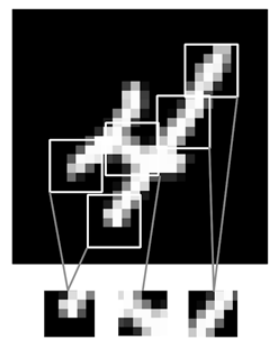
\includegraphics[width=0.25\textwidth]{images/covnet4.png}
    \caption{Imagens podem ser quebradas em padrões locais tais como bordas, texturas, entre outros.}
    \label{fig:quatro}
    \source{Fonte: }
\end{figure}

Essa propriedade permite que as CNN's tenham duas capacidades poderosas e importantes para este trabalho: Os padrões aprendidos são invariantes a sua translação e o aprendizado estabelece uma hierarquia espacial (figura \ref{fig:gato}): Ao aprender um certo padrão, supondo que na borda inferior da imagem, a rede conseguirá reconhecer este em qualquer lugar que ele vier a aparecer; ainda, a primeira camada de convolução aprenderá padrões locais e pequenos, tais como bordas, enquanto que a segunda camada aprenderá padrões maiores feitos dos padrões da primeira camada e assim por diante até a rede como um todo consiga definir conceitos completos como de um animal (Chollet, 2017).

\begin{figure}
    \centering
    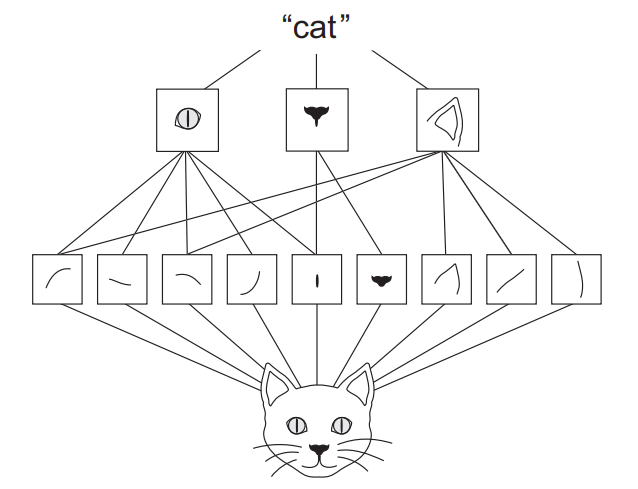
\includegraphics[width=0.6\textwidth]{images/gato.png}
    \caption{A visão forma uma hierarquia espacial de módulos: bordas próximas combinam em objetos como olhos ou orelhas que combinam em um conceitos de mais alto nível como, por exemplo, "gato". }
    \label{fig:gato}
    \source{Fonte: }
\end{figure}

As arquitetura de uma rede convolucional é composta de três camadas principais, chamadas camada de convolução, camada de pool e camadas totalmente conectadas (SINHA; PANDEY; PATTNAIK, 2018). Ilustrada pela figura \ref{fig:passaro}, uma imagem de entrada passa por uma série de camadas de convoluções composta por filtros, posteriormente camadas de pool até chegar por fim na camada classificatória, fornecendo uma classe para a imagem fornecida.

\begin{figure}
    \centering
    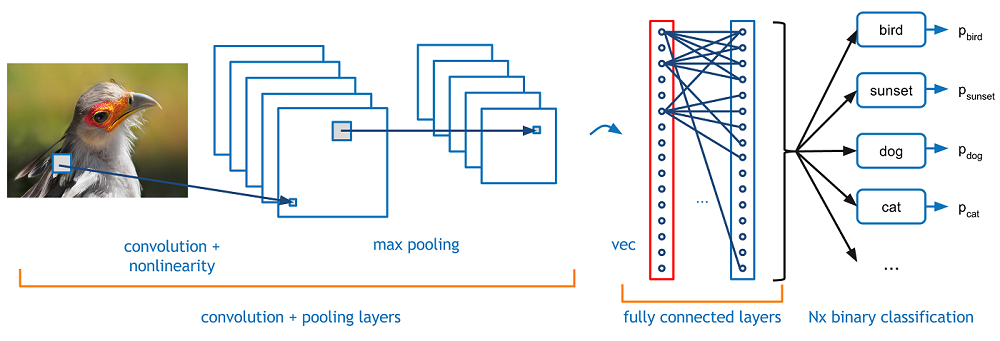
\includegraphics[width=0.8\textwidth]{images/passaro.png}
    \caption{}
    \label{fig:passaro}
    \source{Fonte: }
\end{figure}

\subsubsection{Camadas de Convolução}

A principal funcionalidade das redes neurais convolucionais de aprender padrões e características acontece devido a operação da convolução aplicada através de filtros. Esta operação em imagens digitais acontece sobre um domínio 3-d, largura, altura e profundidade dos canais de cor das imagens. Nessas camadas se constroe um mapa de características (do inglês \textit{feature map}), composto de todas as características obtidas a partir de uma série de filtros aplicadas (CHOLLET, 2017).

\begin{figure}
    \centering
    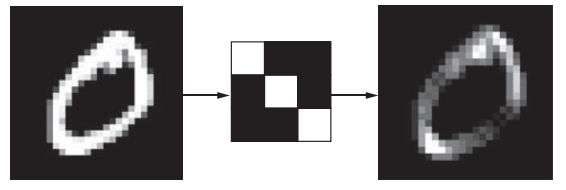
\includegraphics[width=0.5\textwidth]{images/zero.png}
    \caption{}
    \label{fig:zero}
    \source{Fonte: }
\end{figure}

\subsubsection{Camadas de Pool}

Do sentido mineração, estas camadas minimizam a quantidade de informação obtida pelas camadas de convolução de forma a torna-las mais relevantes. Esta operação é também é feita deslizando uma janela sobre a imagem, em busca geralmente dos maiores valores de pixel dentro da janela (figura \ref{fig:maxpool}.  Por exemplo, se após a convolução obtém-se imagens de tamanho 26 x 26, a operação de \textit{max-pooling} diminuirá a mesma para 13 x 13 (CHOLLET, 2017).

\begin{figure}
    \centering
    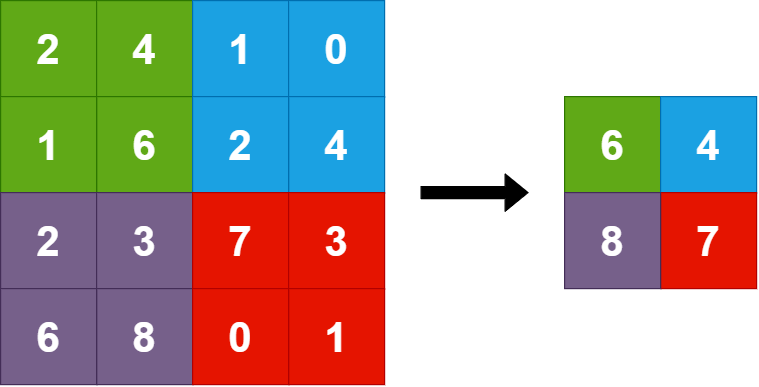
\includegraphics[width=0.5\textwidth]{images/maxpool.png}
    \caption{Operação de Max-Pooling}
    \label{fig:maxpool}
\end{figure}

A motivação para reduzir a quantidade de amostras é reduzir o número de coeficientes do mapa de características a serem processados pela rede. Em poucas palavras as características obtidas tendem a codificar a presença de algum padrão ou conceito, logo é mais informativo olhar sobre a máxima presença de diferentes características do que a média destas espalhadas em muitos valores (CHOLLET, 2017).

\subsubsection{Camadas Classificatória}

Após uma série de camadas de convolução e de pool a imagem se torna uma abstração com uma representação multi dimensional de mapa de características. A partir deste é adicionado uma camada classificatória para fornecer uma resposta informativa ao usuário sobre todas as características abstratas. Esta etapa pode ser entendida como um modelo de aprendizado a parte, que será treinado de acordo com a aplicação do modelo e performance desejada (CHOLLET, 2017).

\subsubsection{Transferência de Aprendizado}

Uma prática comum e altamente eficiente em aplicações com redes neurais convolucionais que possuem pequeno conjunto de dados para treinamento é usar redes pré-treinadas, ao invés de treinar uma. Esta técnica conta com CNN's  previamente treinadas sobre uma grande quantidade de dados, tipicamente para classificação de imagem em larga escala. Se o conjunto de dados fornecido para o treinamento for grande suficiente e abrangente suficiente, possibilitará que a hierarquia espacial das características aprendidas pela rede pré-treinada aja como um modelo genérico de visão do mundo, sendo úteis para diversas aplicações de visão computacional completamente diferentes da tarefa onde foram treinadas - transferência de aprendizado (do inglês \textit{Transfer Learning}) (CHOLLET, 2017).

Há duas formas de utilizar redes pré-treinadas, para extração de características e para ajuste de rede, porém para este trabalho só será relevante o uso como extrator de características. Este método consiste em utilizar o aprendizado obtido de um treinamento prévio para extrair características de novas imagens, geralmente de um contexto diferente. As características obtidas podem então alimentar um classificador que ao ser treinado para uma aplicação específica pode ser usado para fim outro de sua base convolucional em comum (figura \ref{fig:trasnfer}). 

\begin{figure}
    \centering
    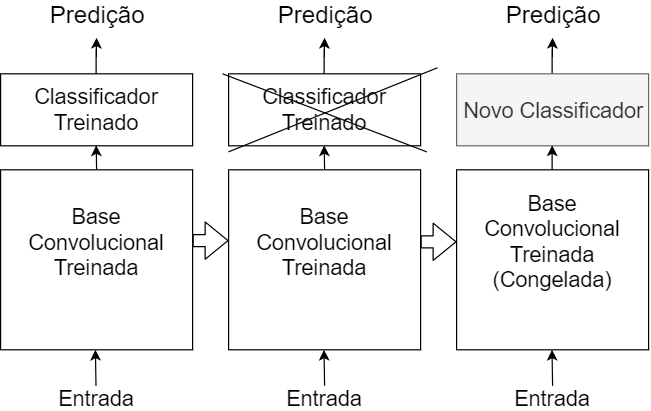
\includegraphics[width=0.7\textwidth]{images/transfer.png}
    \caption{Processo de alterar um modelo para utilização como transferência de aprendizado. A partir de um modelo composto de uma CNN e um classificado é retirado o classificador e colocado outro sobre a mesma base convolutiva, esta mantida sem alteração. }
    \label{fig:trasnfer}
    \source{Fonte:}
\end{figure}

Em geral deve-se evitar reutilizar classificadores, já que as representações aprendidas por esta camada são especificas da aplicação. Para utilizar a base convolutiva, que tem um potencial mais genérico e reutilizável, deve-se atentar para a profundidade das camadas na rede. Já que as camadas mais fundas são mais especializadas, a extração de características para uma aplicação muito diferente pode ser comprometida se os dados novos diferem muito dos dados que esta foi treinada.

\subsection{Rede Neural de Convolução Regional com Máscara}

Do inglês, \textit{Regional Convolutional Neural Network} (\textit{Mask} R-CNN), em tradução literal, esta rede neural foi introduzida como complemento do modelo já renomado para detecção de objetos \textit{Faster} R-CNN. Nesta nova arquitetura foi introduzido o necessário para avançar na ordem de complexidade de segmentação e chegar a segmentação de instâncias. 

Segmentação de instâncias é desafiador pois requer uma detecção correta de todos os objetos em uma imagem enquanto ainda segmenta de forma precisa cada uma de suas instâncias. Esta técnica combina os elementos de detecção e classificação de objetos (figura \ref{fig:seg}) e segmentação semântica. (HE et al, 2018).

\begin{figure}
    \centering
    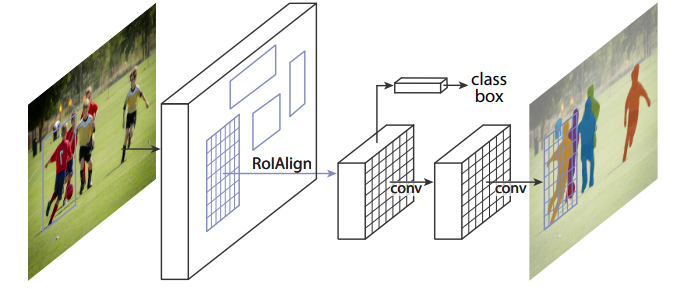
\includegraphics[width=0.6\textwidth]{images/futebol.png}
    \caption{O processo para segmentação de instância da Mask R-CNN}
    \label{fig:futebol}
    \source{Fonte:}
\end{figure}

A estrutura proposta pelo grupo de pesquisa com IA do Facebook, ilustrada na figura \ref{fig:futebol}, recebe uma imagem, detecta a região de interesse e de forma paralela classifica o objeto detectado ao mesmo tempo que melhora sua região delimitadora do objeto detectado (do inglês, \textit{Region of Interest Align} - RoIAlign). Após detectada com precisão a região de interesse este segmento da imagem é passado por uma rede neural convolucional totalmente conectada para prever a segmentação de máscara, pixel a pixel. Alguns exemplos de aplicação podem ser visto na figura \ref{fig:mask}, onde para uma mesma classe, por exemplo pessoa, a rede consegue distinguir diferentes elementos através de máscaras, e ainda delimitar seus limites com um retângulo demarcador.

\begin{figure}
    \centering
    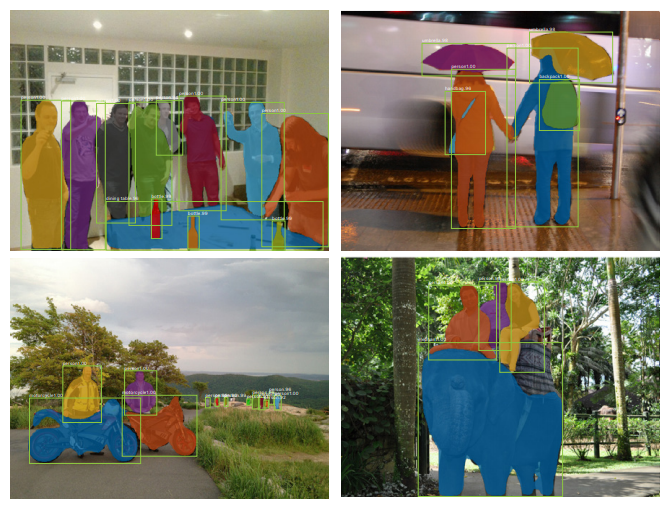
\includegraphics[width=0.6\textwidth]{images/mask.png}
    \caption{Exemplo de resultados obtidos pelo time desenvolvedor da Mask R-CNN aplicado sobre o dataset COCO.}
    \label{fig:mask}
    \source{Fonte:}
\end{figure}


\chapter{Trabalhos Relacionados}
\label{cha:relacionados}

Há diferentes tarefas envolvendo análise de imagens de vestimentas, tais como detecção de roupas, predição de ponto chave, segmentação e obtenção de roupas (traduções livres do inglês \textit{clothes detection}, \textit{landmark prediction}, \textit{clothes segmentation} e \textit{retrieval}) (Deepfashion 2). De acordo com um estudo apresentado por Jia et al. a análise de vestimentas tem recebeu um aumento de atenção contínuo da comunidade de visão computacional nesta década, marcando avançados significativos nas quatro áreas mencionadas.

%Jia et al: https://arxiv.org/ftp/arxiv/papers/1810/1810.10148.pdf

%There are various tasks that analyze clothing images such as clothes detection [2, 14], landmark prediction [15, 19, 17], clothes segmentation [18, 20, 13], and retrieval [7, 5, 14] (deepfashion2).

Trabalhos pioneiros desenvolveram um processo padrão de processamento aperfeiçoado "a mão" (como é chamado, devido a grande complexidade de parâmetros para calibrar), enquanto os processos baseados em \textit{deep learning} não vinham a tona (1503.02391). Para os fins deste trabalho serão mencionados alguns dos trabalhos importantes que marcaram esta trajetória dando ênfase nos que vieram dar suporte no desenvolvimento deste trabalho, nos âmbitos de segmentação de vestimentas e análise de moda envolvendo imagens digitais. 

%lendo: http://www.eecs.qmul.ac.uk/~xiatian/papers/WACV17/DongEtAl_WACV2017.pdf

\section{Segmentação de Vestimentas e Conjuntos de Dados}

*falar do conceito de anotações no ref teórico* 

%acho que não precisa falar de "image retrieval" com cross domain porém: https://arxiv.org/pdf/1709.01784.pdf |||| http://citeseerx.ist.psu.edu/viewdoc/download?doi=10.1.1.370.6283&rep=rep1&type=pdf |||| https://ieeexplore.ieee.org/document/7805463 ||| http://www.nlpr.ia.ac.cn/2012papers/gjhy/gh94.pdf

%image search: https://winstonhsu.info/wp-content/uploads/2017/08/kuo17feature.pdf

%são chamadas de baixo nível para segmentação baseada em estimação de pose e RGB, Lab, MR8, HOG, Boundary Distance [paperdoll] para extração de características. (deep human parsing)

Em 2012 Yamaguchi et al (fashionista) foram pioneiros em aplicar técnicas clássicas de segmentação de imagens para treinar o modelo estatístico CRF para classificação de imagens de pessoas em 53 categorias de vestimentas possíveis. Tendo usado 685 imagens anotadas de pessoas exibindo o que vestiam para treino e teste, obteve 80.1\% de acurácia na análise de pixels e introduziu na literatura o primeiro conjunto de dados ("fashionista") com imagens de vestimentas anotadas disponibilizado online, servindo de referência para diversos estudos subsequentes na área. [20, 5, 7, 3, 14, 12, 21, CFPD, deepfashion2, runway2realway]

%For example, WTBI [5] and DARN [7] have 425K and 182K images respectively. They scraped category labels from metadata of the collected images from online shopping websites, making their labels noisy. In contrast, CCP [20], DeepFashion [14], and ModaNet [21] obtain category labels from human annotators. (DeepFashion2)

O famoso Paperdoll [2], feito buscando melhor acurácia sobre o "fashionista" , implementou descritor de estilo para buscar estilo de roupa semelhantes: um vetor de características descritivas para uma imagem, a partir de técnicas clássicas para extração de características como use RGB, Lab, MR8, HOG, \textit{Boundary Distance}, e \textit{Pose Distance}. Também, observou a problemática da dimensão dos vetores de características para imagem e aplicou PCA para reduzir a dimensão de 39.168 para 441 dimensões. Chegando a ser estado da arte (ATR) melhorou a performance geral do "fashionista" de 77\% para 85\%.

%magic closet [WoW dataset] - não usa CNN para features most suitable clothing by considering the wearing properly and wearing aesthetically principles. We adopted a latent SVM based recommendation model to incorporate the matching rules among visual feature, attribute and occasion within a unified framework. To learn and evaluate the model, we collected a large clothing dataset with full attribute and occasion annotations.

%getting the look - We formulate automatic suggestion of products from online shopping catalogs as a cross-scenario retrieval problem[8], since the query is a real-world image, while the related products are usually presented in a clean and isolated environment - usa fashionista / pose estimation problema com uso das segmentações representam os atributos por color and texture characteristics.

Em cima do "Paperdoll" foram introduzidos diversos estudos com diferentes propostas, muitos dos quais trabalharam em cima de obtenção de imagem. Com grande potencial para vendas online, esta área busca encontrar imagens contendo vestimentas similares a uma determinada imagem, geralmente da rua para loja online [gettingthelook, street2shop, Cross-Domain Image Retrieval]. Runway to Realway (Runway2Realway dataset) entretanto foi além da busca por similaridade ao criar um dataset com 348.598 imagens de desfiles de moda em um período de 15 anos e aplicar o descritor de estilo para treinar um modelo de classificação capaz de medir similaridade entre roupas a partir da opinião humana. O mais atraente deste estudo se fez a capacidade dos descritivos não só acharem imagens semelhantes no banco de imagens, como também estudar a moda ao longo dos anos, percebendo variação de tendências com o tempo. 

Não demorou para que as redes neurais tomassem de conta dos estudos desta área, melhorando a acurácia de seus precursores (deep human parsing, Human parsing Contextualized-CNN) na segmentação e extração de características, assim como criando nossas possibilidades de aplicações. Wheretobuyit (Exact Street2Shop Dataset - 2015), por exemplo, se destacou por ter coletado e categorizado 20.357 imagens de pessoas usando roupas no cotidiano e 404.683 de lojas online, onde 39.479 formavam pares de itens iguais. O estudo que treinou uma CNN para obtenção de características, usou humanos e IA para avaliar sua acurácia e mostrou bons resultado tendo medido a similaridade entre vetores de características através da distância do cosseno. 1703.01386 também se destaca por utilizar o pequeno "fashionista" e chegar numa acurácia nível estado da arte a partir de uma rede pré-treinada no dataset "imagenet". 

%MODANET foi o dataset utilizado no trabalho, logo resolvi dar mais detalhes do estudo

Os conjuntos de dados ModaNeT (2019) e DeepFashion2 (2019) se mostram as opções mais recentes para fundamentar estudos de análises de moda. O primeiro, consiste de uma coleção de 55.176 anotações humanas em imagens a nível de pixel, contendo pessoas em poses diversas e de boa resolução, sobrepondo anotações consideradas fracas do "Paperdoll". Essa coleção foi construída de forma a possibilitar testar os algoritmos estado da arte para detecção e segmentação sobre 13 categorias (\ref{fig:modanet}) que têm sido adotadas como de maior interesse para pesquisa e aplicações de mercado pelo mundo: bolsa, cinto, botas, calçados, sobretudo, vestido, óculos de sol, calças, superior, shorts, saia, chapéu e gravata/cachecol (MODANET, 2019). Diferentemente de outros conjuntos de dados com anotações, ModaNet fornece anotações a nível de píxel sobre cada item de roupa para cada imagem formando um polígono no formato de polígono. Como ilustra a figura \ref{fig:modanet2}, estes criam formas diversas demarcando exatamente cada item e ainda podem ser utilizados para treinar uma rede neural. 

\begin{table}[]
\centering
\begin{tabular}{@{}llll@{}}
\toprule
Categoria         & Descrição                      & Treino & Validação \\ \midrule
Bolsa             & Bolsa                          & 36.699 & 2.155     \\
Cinto             & Cinto                          & 13.743 & 771       \\
Botas             & Botas                          & 7.068  & 691       \\
Calçados          & Calçados                       & 39.364 & 1.617     \\
Sobretudo         & Casaco, jaqueta, terno, blazer & 23.743 & 1.358     \\
Vestido           & Vestido, camisão               & 14.460 & 804       \\
Óculos de sol     & Óculos de sol                  & 8.780  & 524       \\
Calça             & Calças, Calças jeans, leggings & 23.075 & 1.172     \\
Top               & Top, blusa, camiseta, camisa   & 34.745 & 1.862     \\
Shorts            & Shorts                         & 5.775  & 429       \\
Saia              & Saia                           & 10.860 & 555       \\
Chapéu            & Chapéu                         & 5.405  & 491       \\
Cachecol\&Gravata & Cachecol, gravata              & 3.990  & 378       \\ \bottomrule
\end{tabular}
\caption{Distribuiçao das categorias no banco de anotações ModaNet}
\label{table:estat}
\end{table}

\begin{figure}
    \centering
    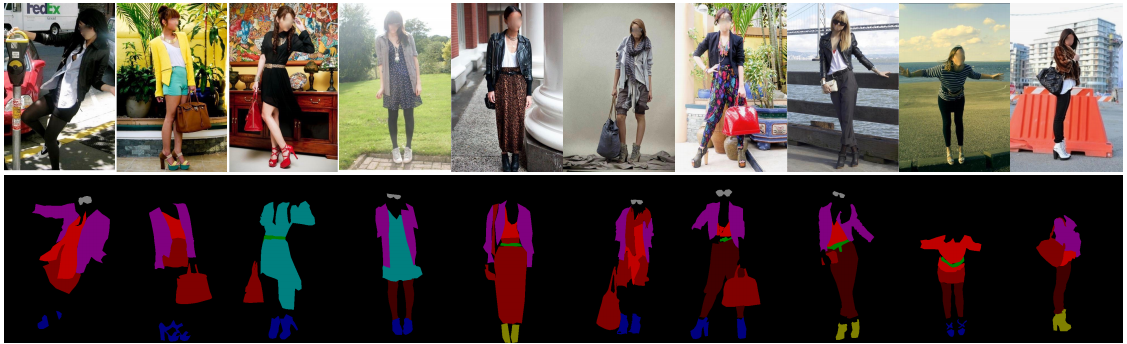
\includegraphics[width=0.85\textwidth]{images/modanet3.png}
    \caption{Exemplos de imagens originais e suas máscaras de segmentação em nível de pixel. A primeira linha mostra uma pessoa e suas vestimentas, enquanto que a segunda linha indica a anotação para cada item colorido para diferenciar categorias.}
    \label{fig:modanet3}
    \source{Fonte:}
\end{figure}

DeepFashion 2 por sua vez, evolução do DeepFashion foca em um construir uma ferramenta completa para entendimento de imagens de moda. Considerado-se estado da arte atualmente, este é composto por 491.000 imagens anotadas com diferentes perspectivas, contendo não só anotações de pixels como também informações de zoom e \textit{landmarks}, por exemplo. Pela primeira vez na literatura é proposto o desafio de estimação de pose de roupas, estendendo o campo de estudo feito até agora sobre poses humanas. Prometendo melhorar a performance da análise de imagens de moda e aplicações no mundo real, este trabalho é pioneiro na estimação de poses de vestimentas com o chamado \textit{landmarks}, apresentando maior aproveitamento do que poses humanas. Ainda, apesar de fazerem uso extensivo da recente arquitetura "Mask R-CNN" e validarem seu benefício, propõem uma nova construída sobre esta, denominada "Match R-CNN". %metrica adotada comparando ambas arquiteturas



\begin{figure}
    \centering
    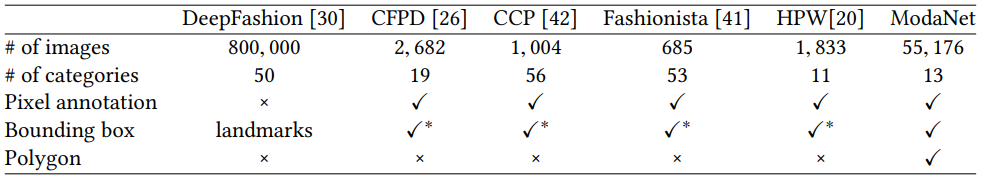
\includegraphics[width=0.9\textwidth]{images/modanet2.png}
    \caption{Comparação do Modanet com outros conjuntos de dados para análise de moda. ✓∗ indica que as anotaçõe não são inclusas no conjunto de dados original. A contagem de categorias exclui as não relacionadas a moda, por exemplo, pele, plano de fundo e null.}
    \label{fig:modanet2}
    \source{Fonte:}
\end{figure}



\section{Análise de Moda Através de Imagens Digitais}
 
 %Hidayati et al. analyze catwalk images from NYC fashion shows to find style trends in high-end fashion [2014].
 
Como mencionado acima, "Runway to Realway" partiu da estimação de pose e análise de vestimenta para concluir que alguns estilos de roupa como estampa floral tinha seu uso variado no tempo. Porém, surgiram estudos mais relevantes voltados para a análise da moda em si através de dados. StreetStyle (2017) procurou analisar moda e estilo de se vestir de milhões de imagens ao redor do mundo por um período de alguns anos. Utilizando aprendizado supervisionado e não supervisionado sobre um dataset próprio, procurou obter atributos de roupas de novas imagens e classificá-las através de aglomerados automáticos para rápida detecção de correlação (t-sne), permitindo análise no formato de mapa. Este trabalho que também utiliza PCA para redução dos vetores de características, obtém bons resultados ao perceber padrões de vestimentas nas maiores cidades do mundo, porém com uma grande limitação, as imagens tratadas foram todas com enquadramento de busto. 

% ? foto do cluster ?

%The base architecture for our CNN pretrained on image classification (on ImageNet ILSVRC2012)  is the “GoogLeNet” architecture [Szegedy et al. 2015]. While several excellent alternatives exist (such as VGG [Simonyan and Zisserman 2014]), GoogLeNet offers a good tradeoff between accuracy on tasks such as image classification [Russakovsky et al. 2015] and speed.


Assim como "StreetStyle", "Learning visual clothing" utilizou agrupamento automático no espaço para entender como sua rede entendia os dados de moda. GeoStyle 1908.11412 (2019), por sua vez, desenvolveu um trabalho em cima do StreetStyle para analisar milhões de imagens e não só entender como as pessoas estavam se vestindo pelo mundo, mas prever eventos responsáveis por mudanças nos padrões, por exemplo, grande número de fotos publicadas com pessoas usando amarelo em 2014 ser relacionado na copa do mundo. 

Diferentemente "Discovering Pictorial Brand association" (2013) buscou analisar associação entre marcas através de imagens digitais. Associação de marca, conceito do marketing, pode ser definido como atitudes ou sentimentos na mente do consumidor em relação a uma marca ou produto, por exemplo, "o que vêm a cabeça de um consumidor quando este pensa na marca Nike?". Esse estudo inovador, utiliza visão computacional no modelo clássico perfeccionado a mão (cor HSV, SIFT e HOG) para buscar similaridade entre imagens e segmentação do que representaria a marca dada uma determinada imagem. Mesmo tendo analisado quase 5 milhões de imagens de 48 marcas, o resultado mostra imagens em baixa resolução, não ficando claro como poderia servir de informação útil. 

\chapter{Desenvolvimento}
\label{cha:meto}

O desenvolvimento do trabalho segue uma série de passos, ilustradas na figura \ref{fig:metodo}, essencialmente construindo uma visão treinada para seleção de peças de roupas durante seu caminho. Partindo de um banco de imagens e suas devidas anotações, há um pré-processamento para torná-las hábeis de serem segmentadas por uma rede neural a qual fornecerá imagens filtradas para serem classificadas de forma não supervisionada pelo algoritmo e gerar um mapa de aglomerados. Dessa forma , neste capítulo é detalhado o processo de desenvolvimento destas etapas, assim como a justificativa para toda decisão tomada nesta metodologia. 

\begin{figure}
    \centering
    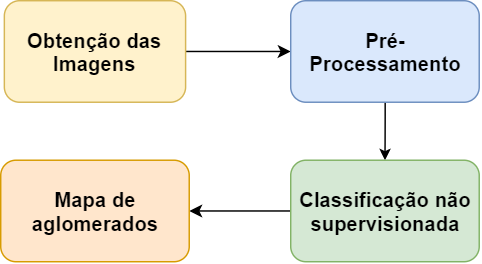
\includegraphics[width=0.55\textwidth]{images/metodo.png}
    \caption{Fases de desenvolvimento}
    \label{fig:metodo}
\end{figure}

\section{Obtenção das Imagens}

Uma vez que o projeto almeja analisar grandes quantidades de imagens de moda e suas características, foi buscado um conjunto de imagens que fossem utilizadas durante todo o processo e fosse qualificado para treinamento e teste do modelo como um todo. Esta busca portanto seguiu duas premissas básicas: Ter disponibilidade livre de custos e ser relacionado a moda. 

\subsection{Imagens para Segmentação}

Os estudos relacionados mencionados, como mencionado, ou utilizam um dataset próprio ou buscam algum já com algum tipo de segmentação para para servir de base e crescer em cima dele. A obtenção das imagens de muitos destes se faz através das redes sociais, partindo do principio que estas estão disponíveis para uso público. Ainda, além da coleta de imagens, estes precisam aplicar segmentação para que as imagens estejam aptas para análise. Porém, devido ao escopo deste projeto e árdua tarefa manual de construir esta estrutura, não se faz possível coletar uma coleção de imagens próprias e realizar sua segmentação. Assim, para que o trabalho mantivesse seu foco na análise das imagens em si, houve necessidade de utilização de um dataset pronto. 

O único conjunto de dados de conhecimento voltado para moda (Runway2Realway dataset) não é público para análise e "DeepFashion", com maior quantidade de imagens anotadas até o momento, requer contato direto para solicitação de acesso. Portanto, seguindo as premissas e limitações mencionadas, a busca resumiu-se ao dataset "ModaNet" ("DeepFashion 2" não havia sido disponibilizado até então). 

Este, já discutido (figura \ref{fig:modanet}), é um banco de anotações livre para estudos de visão computacional, disponível online e construído em cima do "Paperdoll" [ref]. O "Paperdoll" por sua vez contém 1.097.474 de imagens coletadas de uma rede social denominada "Chictopia" [ref], voltada para que seus usuários divulguem fotos de suas roupas, assim construindo uma rede de criadores de estilo. As fotos têm como característica principal pessoas em cenários do cotidiano, de corpo inteiro, em poses diversas, dando enfoque a vestimenta, como ilustra a figura \ref{fig:paperdoll-modanet}. 

\begin{figure}
\centering
  \begin{subfigure}[b]{0.2\textwidth}
  \centering
    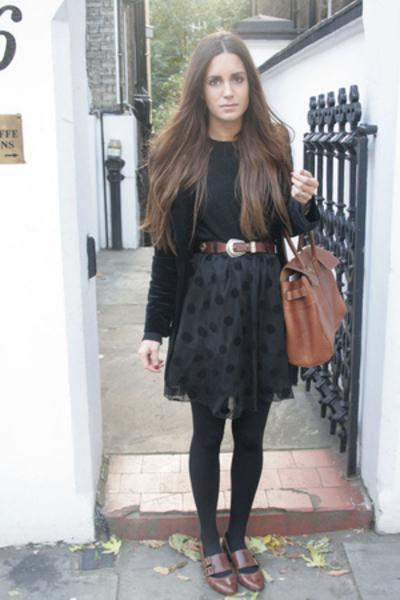
\includegraphics[scale=0.2]{images/paper1.jpg}
    \caption{}
    \label{fig:1}
  \end{subfigure}
  %
  \begin{subfigure}[b]{0.2\textwidth}
  \centering
    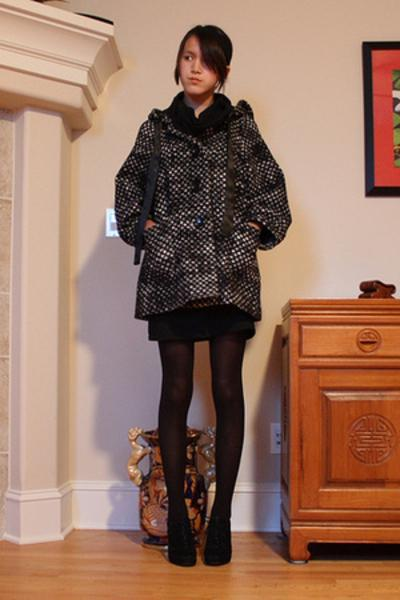
\includegraphics[scale=0.2]{images/paper2.jpg}
    \caption{}
    \label{fig:2}
  \end{subfigure}
  
  \begin{subfigure}[b]{0.2\textwidth}
  \centering
    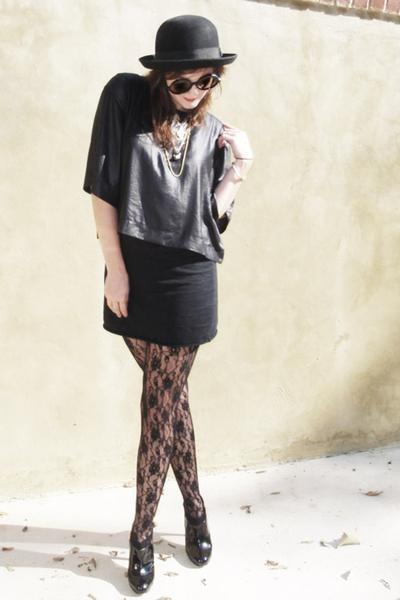
\includegraphics[scale=0.2]{images/paper3.jpg}
    \caption{}
    \label{fig:1}
  \end{subfigure}
  %
  \begin{subfigure}[b]{0.2\textwidth}
  \centering
    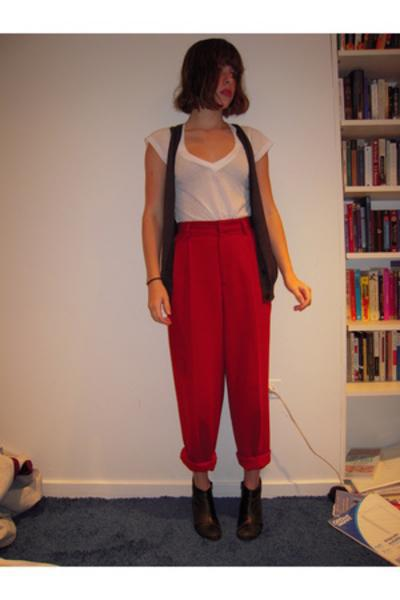
\includegraphics[scale=0.2]{images/paper4.jpg}
    \caption{}
    \label{fig:2}
  \end{subfigure}
  \caption{Exemplo de imagens selecionadas pelo modanet para anotação}
  \source{Fonte: dps}
  \label{fig:paperdoll-modanet}
\end{figure}


O modanet por sua vez coletou dentre as milhares de imagens as com melhor resolução, exposição de vestimentas, garantindo ainda variação de poses e diversificação das classes adotadas. Assim, este é composto por 55.176 imagens no total, 52.377 imagens para treinamento e as 2.799 restantes para validação [ref git], inteiramente anotadas em formato JSON como ilustrado na figura \ref{fig:JSONformat}. Com informações diversas sobre a imagem, como por exemplo: tamanho da imagem, nome, identificador único no banco de imagens do "Paperdoll", assim como as anotações para cada uma, com polígonos que demarcam peças de roupas e os retângulos que demarcam a detecção do objeto na imagem.

\begin{figure}
    \centering
    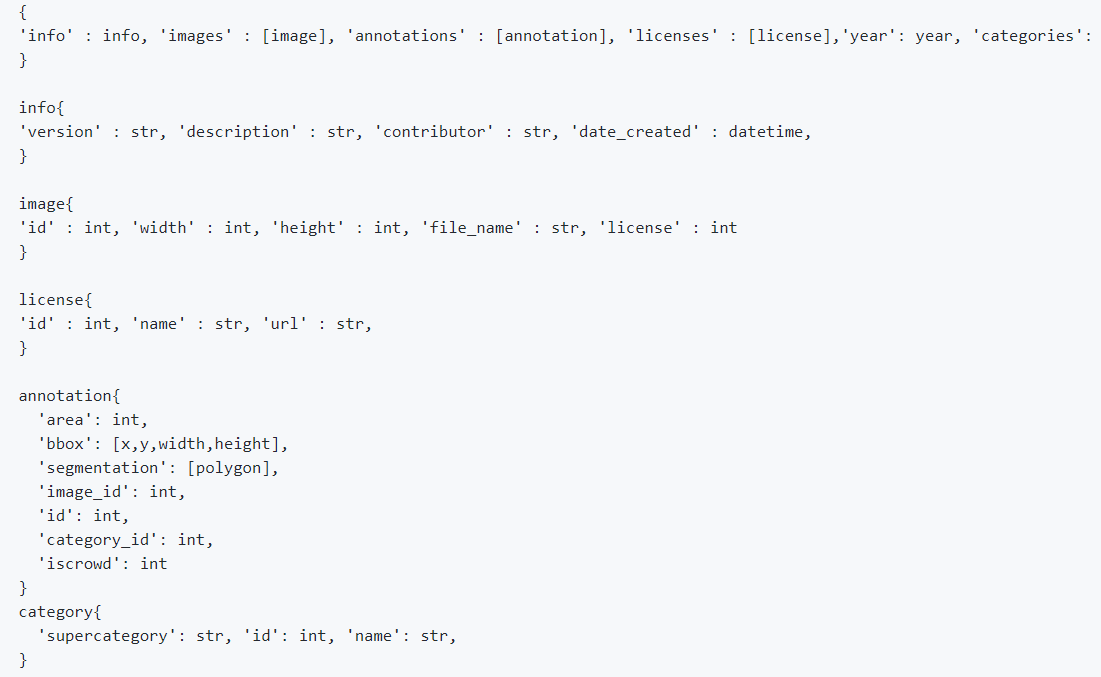
\includegraphics[width=\textwidth]{images/JSONformat.png}
    \caption{Formato JSON de anotação das imagens do modanet}
    \label{fig:JSONformat}
    \source{Fonte: [git do modanet]}
\end{figure}

Dentre o total de anotações do modanet, entretanto, apenas as de treinamento são disponibilizadas para uso público, sendo as de validação incentivadas para que os pesquisadores submetam suas anotações como forma de desafio. Sendo assim, para este trabalho foram adotadas somente as 52.377 imagens já anotadas e feito destas os três conjuntos de anotações necessários para aplicar na rede neural: o de treinamento, com 80\% do total; validação e teste com 10\% cada. 

Com as anotações divididas em três, obteve-se o banco de imagens do "Paperdoll" e, através da sua ferramenta disponibilizada como suporte para acesso a seu banco de imagens, salvou-se apenas as que haviam anotações para os identificadores únicos correspondentes. No fim, aplicando a porcentagem  pré-determinada de separação das anotações, foram obtidas 41.902 imagens para treinamento, 5237 para validação e 5238 para teste, de resolução 400x600 pixels.

\section{Pré-Processamento}

O pré-processamento necessário para as imagens obtidas se faz necessário para minimizar o ruído na análise decorrente do fundo das imagens, isto é, o que não contém roupas. Nesta etapa foram adotadas duas metodologias aplicando a mesma rede neural de segmentação: para segmentar a pessoa presente na imagem, assim como segmentar peças de roupa de uma imagem. Dessa forma o sistema obtém visão para facilitar o uso sobre a moda, ao invés de analisar imagens por completo. 

Para a realização da segmentação das pessoas e das instâncias contidas em cada imagem obtida foi aplicado uma implementação de rede neural do tipo "Mask R-CNN" especialista em detecção de objetos e segmentação. Esta [ref], serve como uma estrutura pronta para aplicações de detecções utilizando imagens ou vídeos, sendo já preparada para receber anotações a nível de pixel de diferentes contextos, assim como as classes correspondentes a cada anotação de roupa.

\subsection{Modelagem das Anotações}

A utilização da "Mask R-CNN" como uma estrutura pronta ajuda na abstração do funcionamento de todas as etapas, sendo necessário configurar e executar somente partes interessadas ao projeto. Do código disponibilizado, a adaptação para novos domínios de aprendizado se faz configurando poucas funções, majoritariamente as funções de carregar as imagens e as devidas suas anotações. Entretanto para vinculação desta rede neural da matterplot com o banco de imagens modanet, se faz necessário modificação do banco modanet para deixar no formato padrão de anotações da rede.

Como ilustra a figura \ref{fig:json-modanet}, o objeto específico anotação possui chave contendo um identificador único da imagem (image\_id), assim como suas instâncias descritas por polígonos, a categoria (category\_id) da instância correspondente etc. Na figura \ref{fig:json-modanet}, uma anotação do modanet contendo uma das possíveis formas de segmentação para uma instância é ilustrada. A chave "segmentation" corresponde a quais pixels pertencem ao item de class "category\_id" de uma imagem identificada por "image\_id". Como cada vetor simboliza um polígono delimitador de pixels para uma peça de roupa, em casos de plural, como no exemplo acima, a instância precisa ser descrita por polígonos separados. Este caso ocorre por diferentes motivos, seja devido a sobreposição de roupa cobrir partes da instância ou devido a limitação 2d da figura.

\begin{figure}[width=\textwidth]
    \centering
    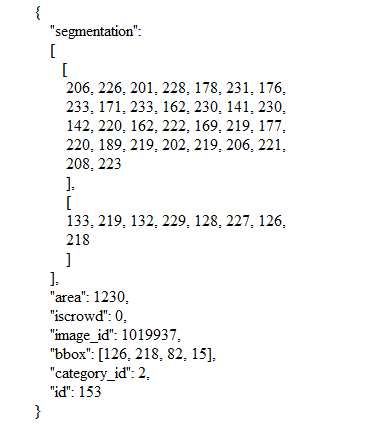
\includegraphics[scale=0.8]{images/json-modanet.png}
    \caption{Exemplo de uma anotação do modanet para a instância "cinto" na imagem 1019937}
    \label{fig:json-modanet}
\end{figure}

Os vetores de segmentação são caracterizados sempre por um valor par de pixels, iniciando com um valor na coordenada X, seguido por um valor Y, até o fim. Ainda, a estrutura da figura \ref{fig:json-modanet} repete-se no banco de anotações para cada nova instância de uma imagem. Para uma imagem contendo, por exemplo, camiseta, calça, bolsa e sapatos anotados, essa estrutura se repetirá para cada uma destas e duas vezes para os sapatos, anotados sempre separados. 

Portanto, devido esta falta de padronização nas anotações de haver várias segmentações separadas para uma mesma imagem, assim como um mesmo vetor conter coordenadas para X e Y, como ainda uma mesma instância ter múltiplos vetores, se fez necessário adaptar as anotações para o padrão da rede neural utilizada. 

A rede Mask RCNN segue um padrão para construção do seu "dataset", composto da vinculação de imagens com suas anotações e classes correspondentes. A adição de imagem no "dataset" espera receber cada imagem descrita pelo conjunto de classes que ela pertence, um número único, o caminho para o arquivo físico, o tamanho em largura e altura, todos o polígonos e a lista de classes disponíveis. A parte responsável por desenhar os polígonos nas imagens, por sua vez, segue o padrão de receber os polígonos das coordenadas X separadamente dos polígonos para as coordenadas Y. 

Para adicionar as imagens ao "dataset", foi criado então um verificador de quantas segmentações há para cada imagem única e salvas de forma unificada para que fossem passadas de uma vez com cada imagem adicionada. A função de desenhar as instâncias por sua vez recebeu um verificador para separar todas as segmentações em vetores de só com coordenadas X e só com coordenadas Y. 

% O resultado dessa modelagem pode ser visto na figura \ref{fig:masks}, mostrando que a rede entende as imagens e suas anotações correspondentes. 

\subsection{Segmentação de Roupas e de Pessoas}

- falar de função custo e especificações matemáticas da rede?

Nesta etapa do pré-processamento a rede neural é utilizada para segmentar roupas e pessoas. A obtenção do banco de imagens "modanet" compõe parte da primeira segmentação, onde a rede é exposta a milhares de imagens contendo diferentes tipos de roupas para aprender a encontrá-las em novas imagens. A segunda segmentação, por sua vez, se torna mais simples devido a redes pré-treinadas para detecção de objetos do cotidiano, incluindo pessoas. 

A "Mask-RCNN", devido sua estrutura pronta para uso, fornece apoio para treinamento com pesos pré-treinados, a fim de agilizar o treinamento em novos domínios. O treinamento de redes neurais complexas como esta podem demorar dias, assim como tunar seus parâmetros ou melhorar sua performance podem ser muito desafiadores. Portanto, matterplot fornece as opções de treinar a rede utilizando os pesos de redes já treinadas em domínios genéricos, como também treinar a rede do início, partindo de pesos aleatórios. Dessa forma, as segmentações realizadas seguiram métodos diferentes, devido a origem do problema. 

Devido a não existência de redes pré-treinadas disponíveis sob o domínio de roupas, se faz necessário treinar a rede como um todo sob este domínio. Para fins comparativos o treinamento foi realizado sobre os pesos pré-treinados das redes "COCO" (Objetos Comuns em contexto, do inglês, \textit{Common Objects in Context}) [ref], "ImageNet" (Desafio de Reconhecimento Visual em Larga Escala ImageNet, do inglês \textit{ImageNet Large Scale Visual Recognition Challenge} - ILSVRC) [ref], assim como partindo de pesos aletórios. 

Os modelos "COCO" e "ImageNet" são redes neurais construídas por organizações com intuito de detectar, classificar e reconhecer cenas de forma geral na área de visão computacional. Tendo 91 e 1000 objetos do cotidiano respectivamente em sua abrangência, estas redes buscam generalizar a visão computacional e contribuir com o avanço do estudo na área disponibilizando seus pesos pós-treinamento. A implementação utilizada da "Mask-RCNN" utiliza os pesos da "COCO" para comparação de performance e se vê melhor em todos os desafios propostos pela plataforma da COCO em 2016, incluindo segmentação de instância, detecção de objetos e detecção de ponto chave de pessoas. 

Uma vez que dentre as classes de cotidiano disponibilizadas por ambas as redes, a classe "pessoa" já está inclusa, para esta segmentação foram aplicados os pesos pré-treinados da COCO para detectar somente pessoas, ignorando qualquer outra classe já conhecida pela rede. 

\section{Classificação Não Supervisionada de Aglomerados}

%deepfashion: https://www.cv-foundation.org/openaccess/content_cvpr_2016/papers/Liu_DeepFashion_Powering_Robust_CVPR_2016_paper.pdf
%The network structure of FashionNet is similar to VGG-16 [25], which has been demonstrated powerful in various vision tasks such as object recognition [25] and segmentation [18].

Com a obtenção e pré-processamento das imagens concluídos, estas finalmente podem ser utilizadas para classificação em aglomerados de forma não supervisionada. Para isso é seguido uma sequência de passos consistindo da extração de características das imagem, redução da dimensão das características, aplicação do t-SNE e no fim a construção do mapa bi-dimensional desejado. Este algoritmo seguido para extração de característica aplicado a transferência de aprendizado tem se provado eficiente e usado para fins didáticos (refs - pyimagenet e ml4a). Neste trabalho, portanto, foi feito uma adaptação em cima da implementação disponibilizada pelo Gene Kogan [ref], cientista que impulsiona o ensino de visão computacional para artistas de forma gratuita.

%https://www.pyimagesearch.com/2017/03/20/imagenet-vggnet-resnet-inception-xception-keras/

\subsection{Extração de Características}

Para a tarefa de classificação de imagens o desafio já citado "ImageNet" para classificação de 1000 classes é considerado [pyimagesearch] referência e tem sido dominado por redes neurais convolucionais e diferentes técnicas de aprendizado profundo desde 2012. Assim sendo, na biblioteca utilizada são disponibilizadas algumas das redes neurais, já treinadas, que apresentaram melhor desempenho no desafio durante os anos, mostrando forte habilidade de generalização para imagens fora do domínio do ImageNet através de transferência de aprendizado  \textit{fine-tuning}).

Como a aplicação de qualquer destes modelos é feita para extração de características das imagens e seus modelos são referências na área, idealmente ao escolher um modelo com alta performance, espera-se uma extração de características satisfatória. Entretanto, para fins de análise, a extração foi submetida a testes utilizando implementações melhoradas de estados da arte passados: "VGG-16" e "Inception\_V3".

A primeira, VGG-16, deriva do projeto VGG da universidade de Oxford [ref] para investigar como a profundidade das redes convolucionais afetam sua acurácia em um sistema de reconhecimento em larga escala. Conseguindo 71,5\% de acurácia no ILSRC de 2012, o modelo apresenta grande capacidade de generalização, chegando a 91,8\% no banco de imagens Caltech-101. Inception V3, do projeto Inception da Google, apresenta uma rede muito mais complexa que a VGG-16, conseguindo atingir 78.2\% de acurácia no ImageNet em 2015, porém com uma redução de 36 vezes na quantidade de parâmetros se comparada com a VGG-16. 

%https://www.robots.ox.ac.uk/~vgg/research/very_deep/
%https://cloud.google.com/tpu/docs/inception-v3-advanced?hl=pt-br

Para aplicar a extração de características, é preciso utilizar as arquiteturas ignorando sua última camada, responsável pela classificação das classes do ImageNet, obtendo-se assim um vetor que descreve a imagem de entrada em sua menor dimensão. Para a VGG-16, ilustrada na figura \ref{fig:vgg16}, o modelo deve ser limitado a camada "fully connected + ReLU" com saída de tamanho 1x4096, ou seja, um vetor contendo 4096 valores descritivos da imagem. Por outro lado, na arquitetura Inception V3, a limitação se dá na camada "AvgPool", resultando em vetor de características do tamanho 1x2048.

\begin{figure}[width=\textwidth]
    \centering
    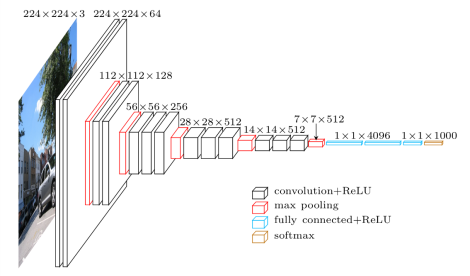
\includegraphics[scale=0.7]{images/vgg16.PNG}
    \caption{Arquitetura do modelo VGG-16}
    \label{fig:vgg16}
\end{figure}

\textbf{editar a imagem do inception v3}

\begin{figure}[width=\textwidth]
    \centering
    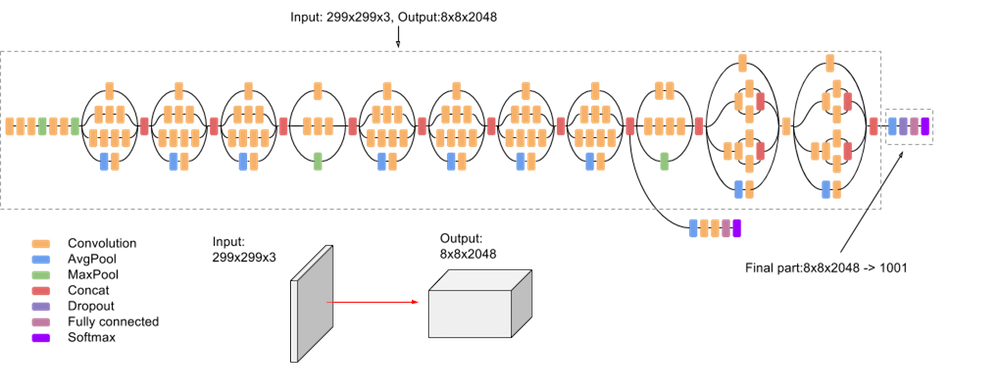
\includegraphics[scale=0.5]{images/inceptionv3.png}
    \caption{Arquitetura do modelo Inception V3}
    \label{fig:inceptionv3}
\end{figure}

Nas arquiteturas \ref{fig:vgg16} e \ref{fig:inceptionv3} também pode ser notado que o tamanho das imagens de entrada nas redes são de baixa qualidade: VGG-16 funciona com imagens coloridas de tamanho 224x224, enquanto que Inception V3 299x299. Esta limitação não contornável é inerente ao desafio do ImageNet, devido a grande quantidade de classe que as redes precisam aprender e ao grande número de parâmetros exigidos delas, trabalhar com imagens pequenas reduz a complexidade da rede. Sendo assim, antes da extração se faz necessário redimensionar todas as imagens para os tamanhos aceitáveis. 

\subsection{Redução da Dimensionalidade e Criação de Aglomerados}
% PCA https://scikit-learn.org/stable/modules/generated/sklearn.decomposition.PCA.html

Uma vez obtidas as características das imagens, são obtidas milhares de valores para cada imagem, sendo ainda assim muitas características a serem tratadas. Para conseguir uma redução ainda maior de dimensão dos descritores, precisa-se reescrever os valores multidimensionais em um espaço de dimensões menor, como por exemplo, através do \textit{Principal Component Analysis}. 

A aplicação de um redutor de dimensionalidade ajuda na síntese dos dados não só na eficiência em tratar menos dados, como também evitando redundância de características. Operar sobre 4096 elementos para cada imagem, por exemplo, é ineficiente em termos de processamento e convergência, logo se estes mesmos dados podem ser representados através de menos dados de forma a não perderem o significado, a performance como um todo é melhorada. Na sua redução PCA não só mantém uma representação fiel aos dados originais, como também evita a redundância de informações para que manter apenas as singulares.

A aplicação do PCA utilizada segue a implementação da biblioteca "scikit-learn", baseada nas implementações de LAPACK ou Halko et al 2009, com decomposição em valores singulares (autovalores e autovetores) completa ou truncada dependendo do tamanho dos dados de entrada e do número de componentes para extrair. Devido a abstração da biblioteca, o uso desta ferramenta PCA requer atenção apenas na regularização dos parâmetros número de componentes e tipo de solucionador. 

%ref sklearn

O número de componentes corresponde a quantidade de componentes para serem mantidos, sendo limitado necessariamente pelo valor mínimo entre o número de amostras de imagens e o número de características obtidas. Este valor, inteiro, pode ser determinado manualmente de forma arbitrária, assim como podendo ser determinado pelo algoritmo de  Minka para detecção automática de dimensões. O solucionador é escolhido automaticamente pela biblioteca a depender do tamanho dos dados de entrada, podendo ser também alterado para versões truncadas ou completas dos algoritmos existentes para PCA.

Após a aplicação do PCA, as dimensões devem ser reduzidas de milhares para a escala de dezenas ou centenas, neste ponto os dados se encontram em um espaço intermediário onde sua redundância foi reduzida, porém para visualizar a semelhança entre as características de duas imagens neste espaço ainda se torna complexo devido a incapacidade humana de correlacionar multi dimensões. Dessa forma, t-SNE pode ser aplicado como outra ferramenta para redução das dimensões dos dados e possibilitar a visualização destes em 2 ou 3 dimensões. 

%ref sklearn

T-SNE é uma ferramenta que converte similaridade entre pontos para probabilidade conjunta e tenta minimizar a divergência de "Kullback-Leibler" entre as probabilidades conjuntas nos espaços de alta e baixa dimensão simultaneamente.  Este algoritmo tem por definição uma função custo não conexa, fazendo com diferentes inicialização resultem em diferentes resultados de visualizações, porém ainda coerentes. Sua aplicação é altamente recomendada a ser utilizada em conjunto com outro métodos de redução de dimensão para dados esparsos, levando os dados de uma alta quantidade de dimensões para um espaço intermediário. Este processo não só agiliza o processamento do algoritmo, como também evita ruídos melhorando a acurácia das novas representações. %For more tips see Laurens van der Maaten’s FAQ [2].

A implementação do t-SNE utilizada aqui também baseou-se na disponibilizada pelo "scikit-learn", tendo também alguns parâmetros para regular na sua execução: Número de componentes, perplexidade, taxa de aprendizado e ângulo. O número de componentes aqui é equivalente ao do PCA, sendo um valor inteiro para a quantidade de dimensões que o algoritmo deve reduzir os dados; A perplexidade refere-se ao número de aglomerados independentes que o t-SNE vai tentar classificar os dados dentro; A taxa de aprendizado equivale a um valor numérico que orienta na convergência do algoritmo, alterações neste valor implicam diretamente na visualização final; Por fim, o ângulo controla a troca de custo entre velocidade e acurácia, para valores baixos a acurácia promete ser melhor, porém demora mais tempo para processar. 

Uma vez configurado todos os parâmetros do PCA e do t-SNE, as imagens podem finalmente serem representadas no espaço bidimensional aglomeradas com suas semelhantes. Em teoria o algoritmo do t-SNE aceita qualquer quantidade de imagens e pode gerar um resultado visual com grandes quantidade de aglomerados. Devido a tantas variáveis e a subjetividade da visualização, as técnicas foram aplicadas repetidas vezes, sob diferentes configurações.

\chapter{Resultados}
\label{cha:resultados}

%Mostre exemplos onde o algoritmo foi BEM SUCEDIDO e também exemplos onde ele foi MAL SUCEDIDO. Isso é ótimo, pois evidencia que você tem consciência das possíveis limitações da sua criação.

Os resultados deste trabalho devem ser descritos por toda sua cadeia de desenvolvimento, muito embora seu resultado final seja claro quanto mapa que deseja-se obter. As imagens utilizadas para ilustração dos resultados são as mesmas anotadas pelo ModaNet, todas compostas por apenas uma pessoa em cena, em cenário cotidiano e de tamanho padrão 600x400 pixels de resolução.

\section{Segmentações}

%- resutado das segmentações de roupas e de pessoas (falando do train)\\
%- mostrar para mask rcnn matriz de confusão etc\\
%- checar a validação da mask rcnn? (cross-validation?)\\

Os experimentos de segmentação aplicados dividem-se nas segmentações de instâncias de vestimentas e na segmentação de pessoas, sendo a primeira a única necessária de treinamento. 

\subsection{Segmentação de Vestimentas}

Antes de treinar a rede neural para aprender a segmentar instâncias de vestimentas, o banco de anotações foi modelado para se adequar a sintaxe exigida pela MASK-RCNN utilizada. O resultado desta alteração, ilustrado na figura \ref{fig:masks}, mostra como a rede entende as anotações a nível de pixel para algumas das imagens do conjunto de treinamento.

\begin{figure}
  \centering
  \begin{subfigure}[b]{\textwidth}
  \centering
    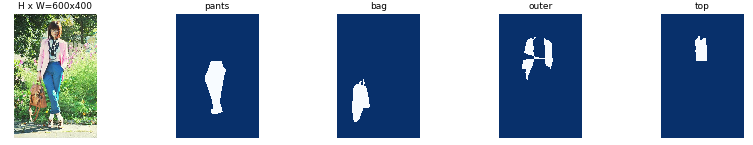
\includegraphics[scale=0.8]{images/mask1.png}
    %\caption{}
    \label{fig:mask1}
  \end{subfigure}
  %
  \centering
  \begin{subfigure}[b]{\textwidth}
  \centering
    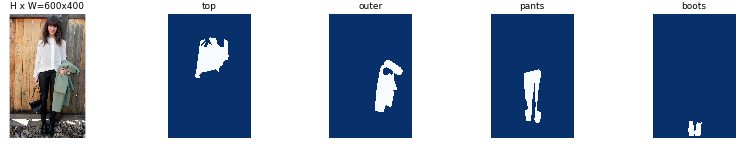
\includegraphics[scale=0.8]{images/mask3.png}
    %\caption{}
    \label{fig:mask3}
  \end{subfigure}
  %
  \centering
  \begin{subfigure}[b]{\textwidth}
  \centering
    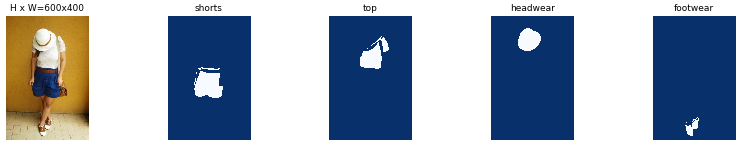
\includegraphics[scale=0.8]{images/mask2.png}
    %yo\caption{}
    \label{fig:mask2}
  \end{subfigure}
  \caption{Inspeção do funcionamento da modelagem de anotações no padrão da rede neural utilizada. As classes ilustradas são respectivamente: Calça, bolsa, sobretudo, blusa, sapatos, shorts e chapéu.}
  \label{fig:masks}
\end{figure}
 
% - o treinamento comparar coco e imagenet
% - falar dos stats do treinamento

O resultado da segmentação se mostra satisfatório para muitos casos, conseguindo detectar muitas instâncias diferentes de roupas. Entretanto, devido a grande quantidade de poses e estilos de roupas presentes nas imagens, muitos exemplos de detecção falham em detectar a roupa por completo ou a instância toda.

Na figura \ref{fig:moda-seg}, podemos ver um exemplo onde as instâncias são detectadas com êxito podendo serem separadas da imagem sem perder seu valor para outros usos. Enquanto que na figura \ref{fig:moda-seg2}, por sua vez, é apresentado um caso onde a bolsa e os sapatos são detectados, porém o vestido é interpretado como vestido, saia e blusa ao mesmo tempo, tendo ainda sido reconhecida uma calça inexistente. 

\begin{figure}
  \centering
  \begin{minipage}[b]{0.3\textwidth}
    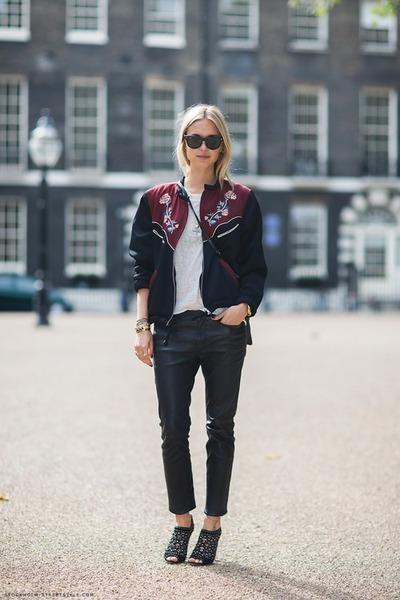
\includegraphics[width=\textwidth]{images/resultados/1060077original.jpg}
    \caption{}
  \end{minipage}
  \hfill
  \begin{minipage}[b]{0.3\textwidth}
    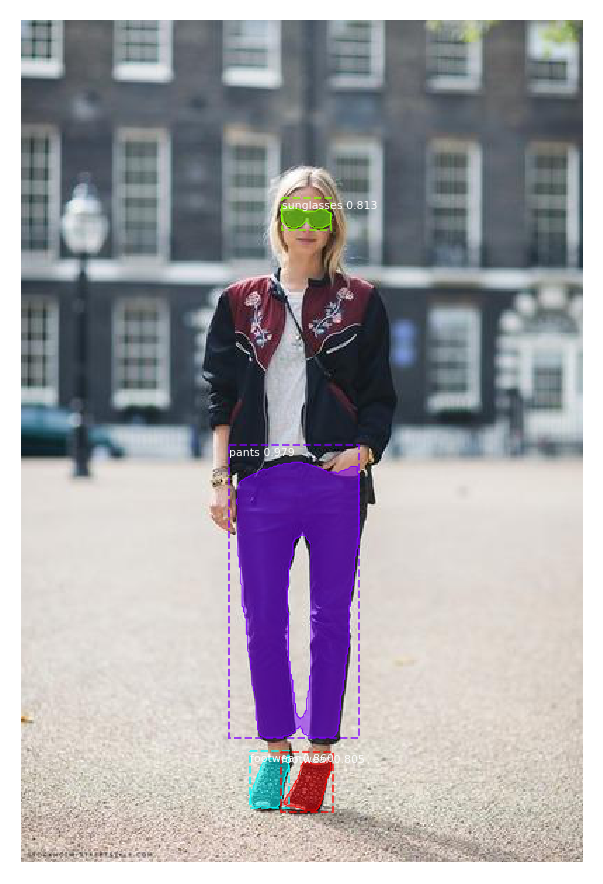
\includegraphics[width=\textwidth]{images/resultados/1060077roupas.png}
    \caption{}
  \end{minipage}
    \hfill
  \begin{minipage}[b]{0.3\textwidth}
    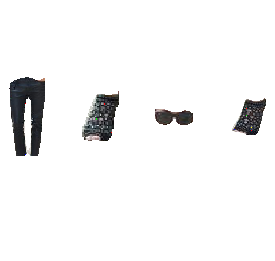
\includegraphics[width=\textwidth]{images/resultados/1.png}
    \caption{}
  \end{minipage}
  \caption{teste}
  \label{fig:moda-seg}
\end{figure}

\begin{figure}
  \centering
  \begin{minipage}[b]{0.48\textwidth}
    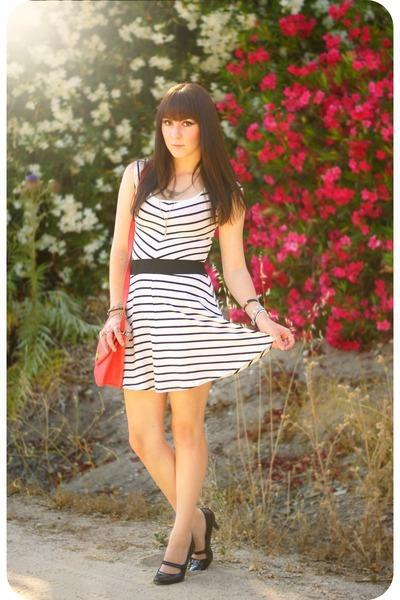
\includegraphics[width=0.8\textwidth]{images/resultados/490842original.jpg}
    \caption{}
  \end{minipage}
  \hfill
  \begin{minipage}[b]{0.48\textwidth}
    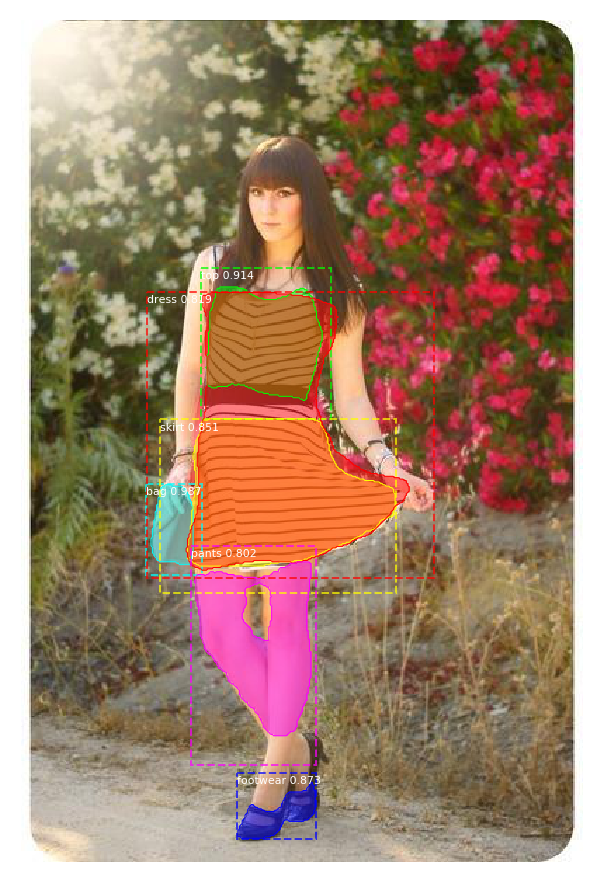
\includegraphics[width=0.8\textwidth]{images/resultados/490842roupas.png}
    \caption{}
  \end{minipage}
    \hfill
  \begin{minipage}[b]{0.7\textwidth}
    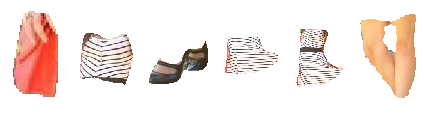
\includegraphics[width=\textwidth]{images/resultados/2.png}
    \caption{}
  \end{minipage}
  \caption{teste}
  \label{fig:moda-seg2}
\end{figure}

\subsection{Segmentação de Pessoas}

A segmentação de pessoas foi aplicada também as imagens do "Paperdoll" obtidas, porém foi executadas na rede sobre os pesos pré-treinados para as classes do cotidiano COCO, que dentre as 80 classes possíveis, limitou-se a reconhecer somente a classe "Pessoa". Este processo de reconhecimento da instância "pessoa" possibilitou a criação de novas imagens contendo somente a instância detectada na imagem original, como ilustrado na figura \ref{fig:person-seg}. 

\begin{figure}
  \centering
  \begin{minipage}[b]{0.3\textwidth}
    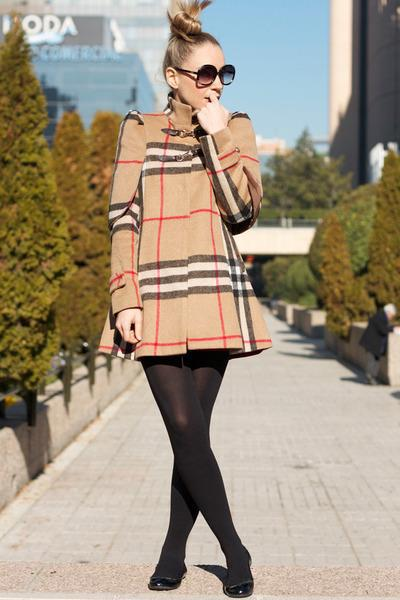
\includegraphics[width=\textwidth]{images/resultados/299206original.jpg}
    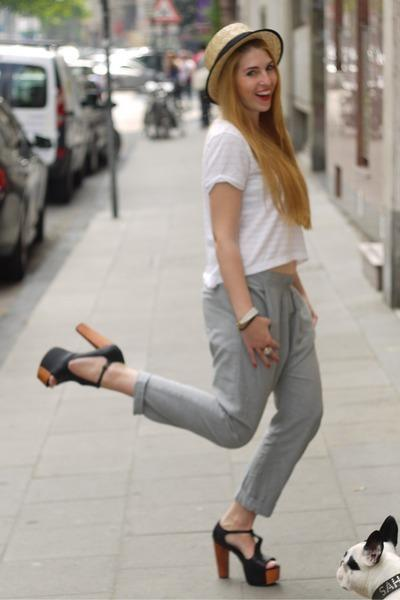
\includegraphics[width=\textwidth]{images/resultados/349322original.jpg}
    \includegraphics[width=\textwidth]{images/resultados/1082993original.jpg}
    \caption{}
  \end{minipage}
  \hfill
  \begin{minipage}[b]{0.3\textwidth}
    \includegraphics[width=\textwidth]{images/resultados/299206person.png}
    \includegraphics[width=\textwidth]{images/resultados/349322person.png}
    \includegraphics[width=\textwidth]{images/resultados/1082993person.png}
    \caption{}
  \end{minipage}
    \hfill
  \begin{minipage}[b]{0.3\textwidth}
    \includegraphics[scale=0.5]{images/resultados/299206mask.jpg}
    \includegraphics[scale=0.5]{images/resultados/349322mask.jpg}
    \includegraphics[scale=0.5]{images/resultados/1082993mask.jpg}
    \caption{}
  \end{minipage}
    \hfill
  \caption{teste}
  \label{fig:person-seg}
\end{figure}

Os resultados das detecções de pessoa conseguem 100\% de acurácia para todas as detecções, porém para criação de um novo banco de imagens a serem utilizadas para análise de moda a rede mostra resultados limitados uma vez que a instância "pessoa" tende a seguir a forma do corpo da pessoa, ignorando muitas vezes partes das roupas e acessórios por sendo utilizados. Mesmo assim, as imagens segmentadas por pessoas foram salvas e aplicadas e testadas na criação dos aglomerados, para reduzir o ruído do plano de fundo. 

Do novo banco de imagens contendo imagens segmentadas, muitos exemplos se mostraram ruidosos como ilustra a figura \ref{fig:segsruins}. Em muitos casos são ruídos pequenos, alterando cores pela imagens, porém em outros casos podem chegar a comprometer por completo a roupa que a pessoa esta vestindo. A razão desta anomalia parece se derivado da baixa resolução das imagens que destas ainda é recriada uma nova imagem de menor resolução ainda - as imagens em \ref{fig:segsruins} possuem resoluções 165x562 e 165x543 respectivamente.

\begin{figure}
  \centering
  \begin{subfigure}[b]{0.4\textwidth}
  \centering
    \includegraphics[width=0.3\textwidth]{images/resultados/159.png}
    %\caption{}
    \label{fig:}
  \end{subfigure}
  %
  \centering
  \begin{subfigure}[b]{0.4\textwidth}
  \centering
    \includegraphics[width=0.3\textwidth]{images/resultados/1532.png}
    %\caption{}
    \label{fig:}
  \end{subfigure}
  \caption{Exemplos onde a segmentação de pessoa gera máscaras ruidosas.}
  \label{fig:segsruins}
\end{figure}


\section{Aglomerados}

%- comparar inception e VGG?

Os resultados dos aglomerados são ilustrados para um conjunto de imagens escolhidas aleatoriamente dentre as imagens sem nenhum pré-processamento, com pessoas segmentadas e por fim para as de instâncias de roupas. 

A figura \ref{fig:originais} ilustra como a imagem fica ao ser redimensionada para a resolução 299x299 exigida pela "Inception V3" e como se parece o vetor de características obtido na saída da rede para a imagem em questão. Idealmente imagens similares entre si deverão apresentar uma proximidade na comparação entre seus vetores. 

\begin{figure}
  \centering
  \begin{subfigure}[b]{\textwidth}
  \centering
    \includegraphics[scale=0.7]{images/resultados/299206menor.png}
    %\caption{}
    \label{fig:}
  \end{subfigure}
  %
  \centering
  \begin{subfigure}[b]{\textwidth}
  \centering
    \includegraphics[scale=0.45]{images/resultados/299206feat.png}
    %\caption{}
    \label{fig:}
  \end{subfigure}
  \label{fig:originais}
\end{figure}

Aplicando uma métrica para medir distância entre vetores, por exemplo, a distância do cosseno, podemos comparar o vetor de características de uma imagem com de várias outras e achar os que apresentam menor distância para verificar a consistência de extração da rede. A figura \ref{fig:compaoriginais} mostra um comparativo de imagens consideradas semelhantes por esta métrica. Ao analisar ambos os casos fica perceptível que as imagens realmente possuem semelhanças de cores, formatos e padrões em geral, muito embora sendo muito influenciadas por regiões não contendo roupa. 

\begin{figure}
  \centering
  \begin{subfigure}[b]{\textwidth}
  \centering
    \includegraphics[scale=0.45]{images/resultados/compaoriginais2.png}
    %\caption{}
    \label{fig:}
  \end{subfigure}
  %
  \centering
  \begin{subfigure}[b]{\textwidth}
  \centering
    \includegraphics[scale=0.45]{images/resultados/compaoriginais3.png}
    %\caption{}
    \label{fig:}
  \end{subfigure}
  \label{fig:originais}
\end{figure}

Ainda assim o t-SNE é gerado para esta coleção de imagens em duas dimensões, figura \ref{fig:tsne1}, para um total de 200 imagens. O mapa gerado utilizou PCA para reduzir o número de características de 2048 para 50, sendo bastante para ser possível classificar as imagens em aglomerados. Para facilitar o entendimento visual, o mapa é colocado em formado de grid na figura \ref{fig:rast1}.

\begin{figure}
    \centering
    \includegraphics[scale=0.5]{images/resultados/tsne2.png}
    \caption{}
    \label{fig:tsne1}
\end{figure}

\begin{figure}
    \centering
    \includegraphics[scale=0.4]{images/resultados/rast1.png}
    \caption{}
    \label{fig:rast1}
\end{figure}

Seguindo o mesmo algoritmo para as imagens de pessoas segmentadas obtém-se desta vez resultados com menor resolução, devido a natureza da criação das imagens serem imagens já serem pequenas, entretanto resultados mais relativos a vestimentas. Na figura \ref{fig:compasegs}, fica mais claro que as imagens consideradas semelhantes agora sofrem menos ruído de outras formas que não o que as pessoas estão usando. 

\begin{figure}
    \centering
    \includegraphics[scale=0.4]{images/resultados/compasegs.png}
    \caption{}
    \label{fig:compasegs}
\end{figure}

O mapa t-SNE obtido para um conjunto também de 200 amostras e com PCA de 50 componentes, é vista na figura \ref{fig:tsne3} e seu respectivo grid na figura \ref{fig:rast2}. O resultado se mostra menos confuso devido haver menos ruído nas imagens, ilustrando aglomerados de roupas semelhantes por cor e estampas. 

\begin{figure}
    \centering
    \includegraphics[scale=0.5]{images/resultados/tsne3.png}
    \caption{}
    \label{fig:tsne3}
\end{figure}

\begin{figure}
    \centering
    \includegraphics[scale=0.4]{images/resultados/rast2.png}
    \caption{}
    \label{fig:rast2}
\end{figure}

Por fim, o processo pode ser levado ao último nível de análise, quando as imagens são instâncias de roupas. Ao aplicar a extração de características sobre estas imagens, é força uma análise feita somente para um tipo de roupa, por exemplo, analisar bolsa, sapatos ou vestidos. A figura \ref{fig:compabolsa} ilustra a análise para bolsas detectadas de imagens aleatórias do banco Paperdoll, que independentemente da baixa resolução, as imagens conseguem ser associadas com suas semelhantes.

\begin{figure}
  \centering
  \begin{subfigure}[b]{\textwidth}
  \centering
    \includegraphics[scale=0.4]{images/resultados/compabolsa.png}
    %\caption{}
    \label{fig:}
  \end{subfigure}
  %
  \centering
  \begin{subfigure}[b]{\textwidth}
  \centering
    \includegraphics[scale=0.4]{images/resultados/compabolsas2.png}
    %\caption{}
    \label{fig:}
  \end{subfigure}
  \caption{Comparativo de bolsas segmentadas.}
  \label{fig:compabolsa}
\end{figure}




\chapter{Conclusões}
\label{cha:conclusoes}

Neste trabalho foi proposto a aplicação de um algoritmo para aglomerar imagens digitais de moda de forma automática de forma a facilitar seu entendimento. A principal motivação para o desenvolvimento deste trabalho é a ineficiência na absorção de coleções de moda durante a grande quantidade de coleções lançadas por ano no mundo e a quantidade de imagens distribuídas em mídias digitais destas criações. A metodologia proposta busca através de aprendizagem de máquina facilitar o entendimento destas imagens a partir de agrupamento automático baseado em suas características. A ferramenta que utiliza segmentação de imagens, busca mais que organizar imagens, determinar características descritivas de vestimentas em geral.

As segmentações que se dividiram em segmentação de pessoas e de instâncias, se mostraram eficientes ao gerar novas imagens para análises que minimizassem a existência de ruído por conta de elementos terceiros nas imagens. A Inception V3 se mostrou eficiente na geração de características coerentes e a análise destas forneceu a obtenção de itens semelhantes próximos. 

Embora os resultados tenham sido ilustrados com imagens de roupas, estas em definitivo não descrevem moda, não tendo nenhuma atrelação com estações, designers ou linha temporal de tendência. Idealmente o trabalho deveria ter sido implementado utilizando imagens de passarela para simular análises reais e comparar como a ferramenta aglomerada itens considerados na moda. Entretanto, para o escopo a solução encontrada se fez a mais recomendada a ser seguida. 

O desenvolvimento do projeto lidou também com limitações de hardware para realizar o treinamento da rede neural de segmentação. Esta que exige uso de GPU, foi treinada utilizando a configuração gratuita fornecido pelo sistema de notebook da Google e obteve sucesso devido não contar com uma quantidade exagerada de anotações. Para o uso de um banco de anotações maior, como o DEEPFASHION 2, o recurso de hardware utilizado não conseguiria suportar.

Como melhorias futuras este projeto poderia ir para a internet e se expandir em um formato de enciclopédia para suas características descritivas das roupas. Para usos que busquem detectar cópia de roupa, por exemplo, ou para fins de comparação entre coleções de moda ou evolução no tempo, a plataforma teria uma quantidade de descritores armazenados e alimentados com o tempo para ajudar no entendimento da moda como um todo. Ainda, os aglomerados poderiam ser gerados de forma interativa no espaço, não no formato de imagem, de forma que um usuário da internet pudesse dar zoom ou analisar melhor os resultados no espaço.

De forma geral, o projeto que surgiu com a ambição de ajudar apenas a melhor visualizar imagens de moda foi elevado a um nível não imaginado ao implementar segmentação. Por mais que enfrentado desafios com a impossibilidade do uso de imagens de passarela, assim como limitações em banco de imagens e anotações disponíveis para treinamento, o estudo cumpre suas metas estabelecidas com o mérito de ter conseguido fazer o melhor para cumprir o escopo.

\newpage
\bibliography{referencias}

\end{document}
